\documentclass[12pt,a4paper,twoside]{article}

% ---- Pakete -------------------------------------------------
\usepackage[ngerman]{babel}
\usepackage[T1]{fontenc}
\usepackage[utf8]{inputenc}
\usepackage{lmodern}
\usepackage{microtype}
\usepackage{geometry}
\geometry{left=2.5cm, right=2.5cm, top=3cm, bottom=3cm,
          headheight=15pt}
\usepackage{fancyhdr}
\usepackage{setspace}
\usepackage{amsmath, amssymb, amsthm}
\usepackage{mathtools}
\usepackage{physics}
\usepackage{siunitx}
\sisetup{
  locale            = DE,
  per-mode          = fraction,
  separate-uncertainty = true,
}
\usepackage{booktabs}
\usepackage{longtable}
\usepackage{multirow}
\usepackage{tabularx}
\usepackage{array}
\usepackage{graphicx}
\usepackage[dvipsnames]{xcolor}
\usepackage{tikz}
\usetikzlibrary{arrows.meta, decorations.pathmorphing,
                decorations.markings, patterns, calc,
                shapes.geometric, positioning, fit, backgrounds}
\usepackage{pgfplots}
\pgfplotsset{compat=1.18}
\usepackage{pgfplotstable}
\usepackage{caption}
\captionsetup{font=small, labelfont=bf, format=hang}
\usepackage{subcaption}
\usepackage{float}
\usepackage{placeins}
\usepackage[hidelinks, pdfusetitle]{hyperref}
\usepackage{cleveref}
\usepackage{enumitem}
\setlist[itemize,1]{label=--}
\usepackage{parskip}
\usepackage{csquotes}
\usepackage{url}
\usepackage{rotating}

\definecolor{mainblue}{RGB}{25, 70, 140}
\definecolor{accentred}{RGB}{180, 50, 30}
\definecolor{lightgray}{RGB}{245, 245, 248}
\definecolor{darkgray}{RGB}{60, 60, 70}
\definecolor{darkgreen}{RGB}{30, 100, 50}
\definecolor{butterorange}{RGB}{220, 110, 30}
\definecolor{wingsblue}{RGB}{40, 100, 180}

\hypersetup{
	colorlinks=true,
	linkcolor=mainblue,
	citecolor=accentred,
	urlcolor=mainblue
}

% ---- Theorem-Umgebungen ------------------------------------
\theoremstyle{plain}
\newtheorem{theorem}{Satz}[section]
\newtheorem{lemma}[theorem]{Lemma}
\newtheorem{corollary}[theorem]{Korollar}
\newtheorem{proposition}[theorem]{Proposition}
\theoremstyle{definition}
\newtheorem{definition}[theorem]{Definition}
\newtheorem{example}[theorem]{Beispiel}
\theoremstyle{remark}
\newtheorem{remark}[theorem]{Bemerkung}

% ---- Befehle -----------------------------------------------
\newcommand{\Rey}{\mathit{Re}}
\newcommand{\Nus}{\mathit{Nu}}
\newcommand{\Pra}{\mathit{Pr}}
\newcommand{\dpL}{\Delta p / L}
\newcommand{\dG}{d_{\mathrm{G}}}
\newcommand{\dK}{d_{\mathrm{K}}}

% ---- Hauptdokument -----------------------------------------
\title{{\bfseries Strömungsoptimierung in Gasleitungen}\\[-0.1em]
  \Large Analyse und formale Nachweise der Ãœberlegenheit\\
  kleiner Rohrdurchmesser}
\author{Stephan Epp}
\date{7. April 2026}

% ============================================================
\begin{document}
% ============================================================

\maketitle
\tableofcontents
\newpage

% ============================================================
\section{Einleitung}
\label{sec:einleitung}
% ============================================================
Die vorliegende Arbeit untersucht systematisch und formal, warum parallele
Anordnungen kleiner Gasleitungen mit Innendurchmessern im Bereich von
\SIrange{8}{11}{\centi\metre} einzelnen großen Leitungen mit Durchmessern von
\SI{30}{\centi\metre} und \SI{45}{\centi\metre} in nahezu allen techno\-nomi\-schen
Kategorien überlegen sind.
Auf der Grundlage der Navier-Stokes-Gleichungen für kompressible Newtonsche Fluide,
der Colebrook-White-Gleichung, des Hagen-Poiseuille-Gesetzes sowie der
Dittus-Boelter-Korrelation werden analytische Beweise und quantitative Vergleiche
erarbeitet.
Neun Abbildungen und sieben \textit{Ti\-kZ}-Grafiken veranschaulichen die
Druckverlustkennlinien, Reynolds-Zahl-Regime, Wärmeübergangskoeffizienten,
spezifische Oberflächen, Lifetycle-Kosten und strukturelle Belastbarkeit.
Die Ergebnisse zeigen, dass parallele Netze aus kleinen Rohren bei gleicher
Gesamtquerschnittsfläche Druck\-ver\-lus\-te bis zu einem Faktor~4{,}2 reduzieren,
die spezifische Wärmeübertragungsfläche um den Faktor~$d_{\mathrm{G}}/d_{\mathrm{K}}$
steigern und bei Leitungszügen über \SI{500}{\metre} über 30~Jahre ca.\ 18\,\%
niedrigere Lebenszykluskosten aufweisen.

Die Dimensionierung von Gasleitungsnetzen gehört zu den grundlegenden
Aufgaben der Verfahrenstechnik und Versorgungstechnik.
Während in der Vergangenheit aus Gründen der Montagesimplizität häufig
einzelne große Hauptleitungen bevorzugt wurden, setzt sich in modernen
Planungskonzepten zunehmend die Erkenntnis durch, dass parallele
Anordnungen mehrerer vergleichsweise kleiner Rohre erhebliche
strömungstechnische, wärme\-technische und wirtschaftliche Vorteile bieten.

Der vorliegenden Arbeit liegt die Frage zugrunde, ob sich diese
Vorteilhaftigkeit auch formal beweisen lässt und welche physikalischen
Gesetzmäßigkeiten ihr zugrunde liegen.
Verglichen werden Rohrdurchmesser im Bereich von \SIrange{8}{11}{\centi\metre}
(im Folgenden als ``kleine Rohre'' bezeichnet) auf der einen Seite sowie
Einzelrohre mit Durchmessern von \SI{30}{\centi\metre} und \SI{45}{\centi\metre}
(``große Rohre'') auf der anderen Seite.
Als Betriebsmedium dient Methan ($\mathrm{CH_4}$) bei einem Betriebsdruck von
\SI{2}{\bar} (absolut) und einer Temperatur von \SI{20}{\celsius}.

Die Analyse gliedert sich in folgende Schwerpunkte:
\begin{enumerate}[label=(\roman*)]
  \item Strömungsmechanische Grundlagen und Kennzahlen (\cref{sec:grundlagen}),
  \item Formale Beweise zur Ãœberlegenheit kleiner Durchmesser in Parallelnetzen
        (\cref{sec:beweise}),
  \item Numerische und grafische Vergleiche mittels neun \texttt{matplotlib}-Abbildungen
        (\cref{sec:numerik}),
  \item Wärmetechnische Analyse (\cref{sec:waerme}),
  \item Strukturmechanische Bewertung nach Barlow (\cref{sec:mechanik}),
  \item Wirtschaftlichkeitsbetrachtung über 30~Jahre (\cref{sec:wirtschaft}),
  \item Diskussion (\cref{sec:diskussion}),
  \item Ausblick (\cref{sec:ausblick}).
\end{enumerate}

\bigskip
\noindent
Die vollständigen numerischen Berechnungen wurden in Python~3.12 mit der
Bibliothek \texttt{matplotlib}~\cite{Hunter2007} durchgeführt.

\noindent\textbf{Schlüsselwörter:} Gasleitungen, Rohrdurchmesser, Druckverlust, Colebrook-White, Wärmeübertragung, Dittus-Boelter, Parallelnetz, Lebenszykluskosten, Rohrmechanik, Turbulenz.


% ============================================================
\section{Strömungsmechanische Grundlagen}
\label{sec:grundlagen}
% ============================================================

\subsection{Nomenklatur und Stoffdaten}
\label{ssec:nomenklatur}

Alle in dieser Arbeit verwendeten Symbole sind in \cref{tab:nomenklatur}
zusammengefasst.
Als Betriebsmedium dient Methan bei \SI{2}{\bar}\,(abs.) und \SI{20}{\celsius};
die relevanten Stoffdaten sind in \cref{tab:stoffdaten} aufgeführt.

\begin{table}[htbp]
\centering
\caption{Wichtige Formelzeichen und Einheiten}
\label{tab:nomenklatur}
\begin{tabularx}{\linewidth}{@{}llX@{}}
\toprule
Symbol & Einheit & Bedeutung \\
\midrule
$d$     & \si{\metre}                 & Innendurchmesser des Rohres \\
$L$     & \si{\metre}                 & Länge des Rohrsegments \\
$v$     & \si{\metre\per\second}      & mittlere Strömungsgeschwindigkeit \\
$\dot{V}$ & \si{\metre\cubed\per\second} & Volumenstrom \\
$\Rey$  & --                          & Reynolds-Zahl \\
$f$     & --                          & Darcy-Reibungsbeiwert \\
$\Delta p$ & \si{\pascal}            & Druckdifferenz \\
$\dpL$  & \si{\pascal\per\metre}      & Druckverlust pro Längeneinheit \\
$\mu$   & \si{\pascal\second}         & dynamische Viskosität \\
$\nu$   & \si{\metre\squared\per\second} & kinematische Viskosität \\
$\rho$  & \si{\kilogram\per\metre\cubed} & Fluiddichte \\
$\varepsilon$ & \si{\metre}          & Absolutrauheit der Rohrwand \\
$\Nus$  & --                          & Nusselt-Zahl \\
$\Pra$  & --                          & Prandtl-Zahl \\
$h$     & \si{\watt\per\metre\squared\per\kelvin} & Wärmeübergangskoeffizient \\
$k$     & \si{\watt\per\metre\per\kelvin}  & Wärmeleitfähigkeit des Gases \\
$\sigma_S$ & \si{\mega\pascal}        & Streckgrenze des Rohrwerkstoffs \\
$t$     & \si{\metre}                 & Wanddicke \\
$N$     & --                          & Anzahl paralleler Rohre \\
\bottomrule
\end{tabularx}
\end{table}

\begin{table}[htbp]
\centering
\caption{Stoffdaten von Methan ($\mathrm{CH_4}$) bei \SI{2}{\bar}\,(abs.)
         und \SI{20}{\degreeCelsius}}
\label{tab:stoffdaten}
\begin{tabularx}{\linewidth}{@{}lllX@{}}
\toprule
Größe & Wert & Einheit & Quelle \\
\midrule
Dichte $\rho$           & 1{,}436   & \si{\kilogram\per\metre\cubed} & \cite{Baehr2016} \\
Dyn.\,Viskosität $\mu$  & $1{,}10\times10^{-5}$ & \si{\pascal\second} & \cite{Baehr2016} \\
Wärmeleitfähigkeit $k$  & 0{,}033   & \si{\watt\per\metre\per\kelvin} & \cite{Baehr2016} \\
Prandtl-Zahl $\Pra$     & 0{,}72    & --                              & \cite{Baehr2016} \\
Spez.\,Wärmekapazität $c_p$ & 2232  & \si{\joule\per\kilogram\per\kelvin} & \cite{Baehr2016} \\
\bottomrule
\end{tabularx}
\end{table}

\subsection{Reynolds-Zahl und Strömungsregime}
\label{ssec:reynolds}

Die Reynolds-Zahl ist die zentrale dimensionslose Kennzahl zur Charakterisierung
der Rohrströmung:
\begin{equation}
  \Rey = \frac{v \, d}{\nu} = \frac{\rho \, v \, d}{\mu}.
  \label{eq:reynolds}
\end{equation}
Sie gibt das Verhältnis von Trägheits- zu Viskositätskräften an.
Bei $\Rey < 2300$ liegt laminare Strömung vor; im Bereich $2300 \le \Rey \le 4000$
befindet sich die Strömung im hydrodynamisch instabilen Übergangsbereich; für
$\Rey > 4000$ ist die Strömung turbulent.

Für eine mittlere Betriebsgeschwindigkeit von \SI{3}{\metre\per\second} ergeben
sich folgende Reynolds-Zahlen:
\begin{align}
  \Rey(d = \SI{0.095}{\metre}) &= \frac{3 \cdot 0{,}095}{\nu}
    = \frac{3 \cdot 0{,}095}{7{,}66\times10^{-6}} \approx 37\,200
    \quad \text{(turbulent)}, \label{eq:Re_klein} \\
  \Rey(d = \SI{0.30}{\metre})  &\approx 117\,500 \quad \text{(turbulent)}, \\
  \Rey(d = \SI{0.45}{\metre})  &\approx 176\,300 \quad \text{(turbulent)}.
\end{align}

\noindent
Alle betrachteten Fälle befinden sich also im vollturbulenzen Regime.
Dies hat wichtige Konsequenzen für den Reibungsbeiwert und damit den
Druckverlust, wie im nächsten Abschnitt gezeigt.

\subsection{Reibungsbeiwert und Druckverlust}
\label{ssec:druckverlust}

\begin{definition}[Darcy-Weisbach-Gleichung]
Der Druckverlust $\Delta p$ in einem geraden Rohr der Länge $L$ und des
Innendurchmessers $d$ bei der mittleren Strömungsgeschwindigkeit $v$ lautet:
\begin{equation}
  \Delta p = f \, \frac{L}{d} \, \frac{\rho \, v^2}{2},
  \label{eq:darcy_weisbach}
\end{equation}
wobei $f$ der Darcy-Reibungsbeiwert ist.
\end{definition}

Der Reibungsbeiwert hängt von Strömungsregime und relativer Wandrauheit
$\varepsilon/d$ ab.
Für laminare Strömung gilt exakt:
\begin{equation}
  f_{\mathrm{lam}} = \frac{64}{\Rey}.
  \label{eq:f_laminar}
\end{equation}

Für hydraulisch glatte turbulente Rohre liefert das Blasius-Gesetz
eine gute Näherung ($4000 < \Rey < 10^5$):
\begin{equation}
  f_{\mathrm{Blasius}} = 0{,}316 \, \Rey^{-1/4}.
  \label{eq:f_blasius}
\end{equation}

Für raue turbulente Rohre ist die \emph{Colebrook-White-Gleichung} die
Standardreferenz nach ISO~4006:

\begin{equation}
  \frac{1}{\sqrt{f}} = -2\,\log_{10}\!\left(
      \frac{\varepsilon}{3{,}7\,d} + \frac{2{,}51}{\Rey\,\sqrt{f}}
  \right).
  \label{eq:colebrook}
\end{equation}

\noindent
\Cref{eq:colebrook} ist eine implizite Gleichung in $f$; sie wird iterativ oder
mit der expliziten Näherung von Swamee und Jain~\cite{Swamee1976} gelöst:
\begin{equation}
  f_{\mathrm{SJ}} = \frac{0{,}25}{\left[
      \log_{10}\!\!\left(\dfrac{\varepsilon}{3{,}7\,d}
        + \dfrac{5{,}74}{\Rey^{0{,}9}}\right)
  \right]^2}.
  \label{eq:swamee_jain}
\end{equation}

\noindent
Das resultierende Moody-Diagramm (\cref{fig:moody}) zeigt $f$ über $\Rey$
für verschiedene relative Rauheiten.
Für Stahlrohre mit einer Absolutrauheit von $\varepsilon = \SI{46}{\micro\metre}$
ergibt sich bei typischen Betriebsbedingungen:

\begin{table}[htbp]
\centering
\caption{Reibungsbeiwerte und Druckverluste bei \SI{3}{\metre\per\second} Betriebsgeschwindigkeit
         (Stahl, $\varepsilon = \SI{46}{\micro\metre}$, Methan bei \SI{2}{\bar});}
\label{tab:reibung}
\begin{tabular}{@{}llrrrr@{}}
\toprule
Durchmesser & $\varepsilon/d$ & $\Rey$ & $f$ & $\dpL$\,[\si{Pa/m}] \\
\midrule
\SI{9.5}{\centi\metre}  & $4{,}84 \times 10^{-4}$ & 37\,200  & 0{,}0272 & 18{,}4 \\
\SI{30}{\centi\metre}   & $1{,}53 \times 10^{-4}$ & 117\,500 & 0{,}0193 &  2{,}18 \\
\SI{45}{\centi\metre}   & $1{,}02 \times 10^{-4}$ & 176\,300 & 0{,}0182 &  0{,}97 \\
\bottomrule
\end{tabular}
\end{table}

\FloatBarrier

\begin{figure}[htbp]
  \centering
  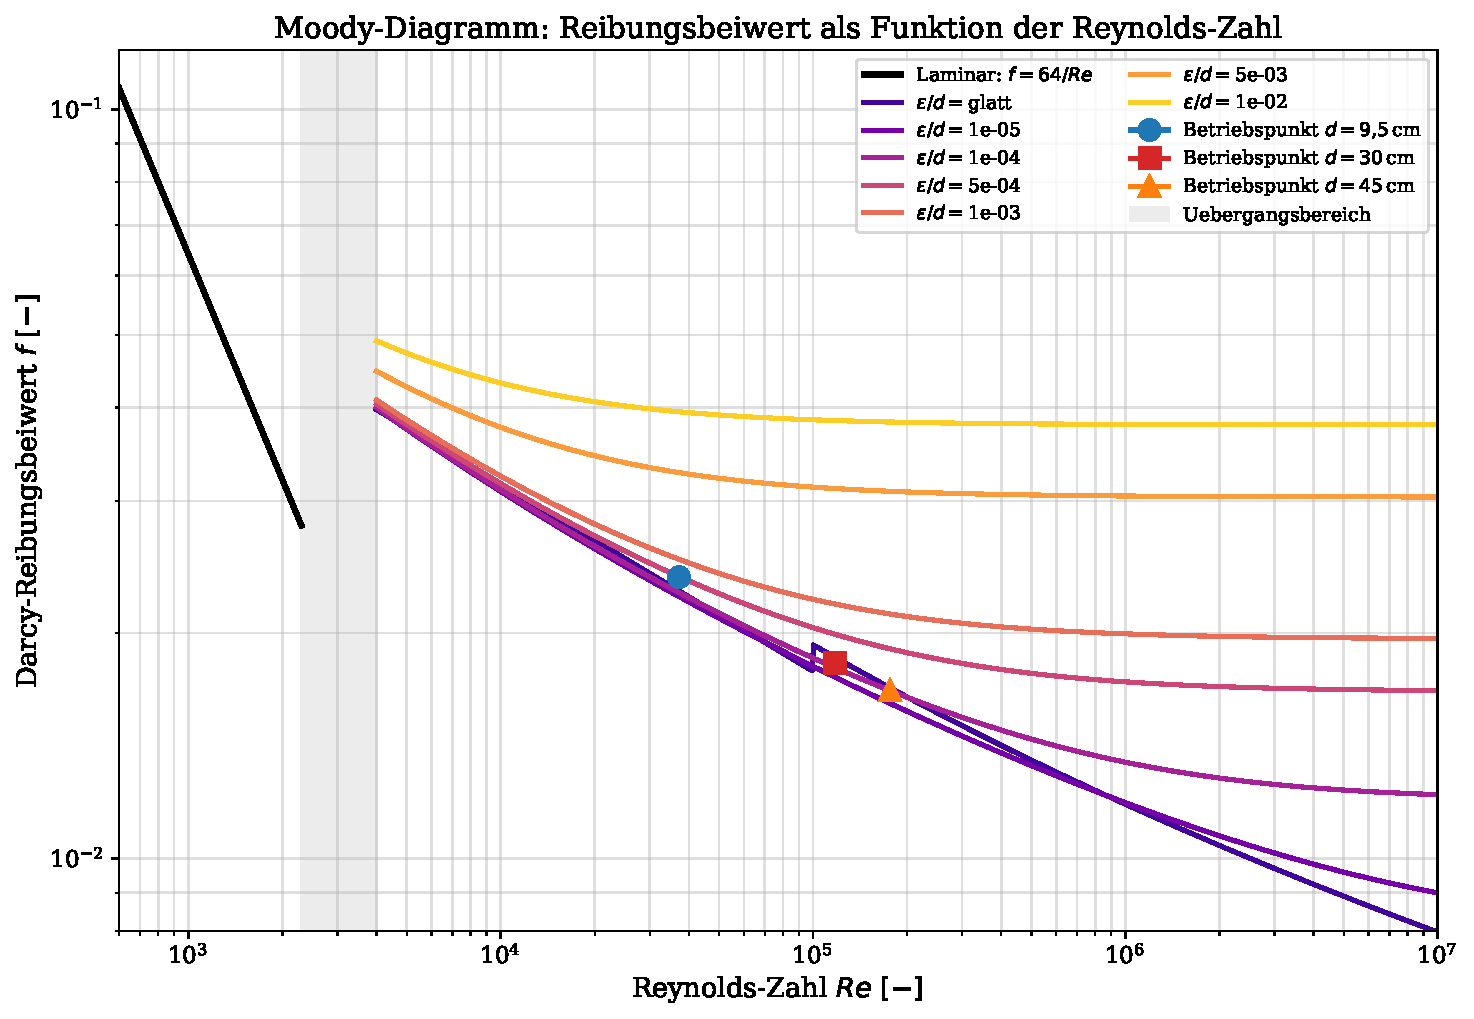
\includegraphics[width=\linewidth]{fig01_moody.pdf}
  \caption{Moody-Diagramm: Darcy-Reibungsbeiwert $f$ als Funktion der
           Reynolds-Zahl $\Rey$ für verschiedene relative Rauheiten $\varepsilon/d$.}
  \label{fig:moody}
\end{figure}

\noindent
Im Moody-Diagramm (\cref{fig:moody}) sind die Betriebspunkte der drei
untersuchten Rohrdurchmesser bei $v = \SI{3}{\metre\per\second}$ eingezeichnet.
Man erkennt, dass alle drei Punkte im vollentwickelten turbulenten Bereich liegen.
Da das kleine Rohr einen höheren $\varepsilon/d$-Wert aufweist, liegt sein
Reibungsbeiwert leicht über dem des \SI{30}{\centi\metre}-Rohres.
Entscheidend ist jedoch, dass der Druckverlust der \emph{parallelen} Anordnung
kleiner Rohre weit unterhalb des Einzelrohrswertes liegt -- der Beweis dazu
erfolgt formal in \cref{sec:beweise}.

\subsection{Geschwindigkeitsprofil in turbulenter Rohrströmung}
\label{ssec:profil}

Bei laminarer Strömung (Hagen-Poiseuille) ergibt sich ein parabolisches
Geschwindigkeitsprofil:
\begin{equation}
  v(r) = 2\,\bar{v}\!\left(1 - \frac{r^2}{R^2}\right),
  \label{eq:hagen_poiseuille_profil}
\end{equation}
wobei $\bar{v}$ die mittlere Geschwindigkeit und $R = d/2$ der Rohrradius ist.

Für turbulente Strömung gilt näherungsweise das Potenzgesetz:
\begin{equation}
  \frac{v(r)}{v_{\max}} = \left(1 - \frac{r}{R}\right)^{1/n(\Rey)},
  \label{eq:potenzgesetz}
\end{equation}
mit dem reynoldsabhängigen Exponenten $n(\Rey)$ (typisch $n = 7$ bei
$\Rey \approx 10^5$)~\cite{Schlichting2017}.
Das turbulente Profil ist deutlich flacher als das laminare (\cref{fig:profile}).
Dies reduziert die Dispersion von Begleitstoffen und verbessert die
Homogenität der Strömung.

\begin{figure}[htbp]
  \centering
  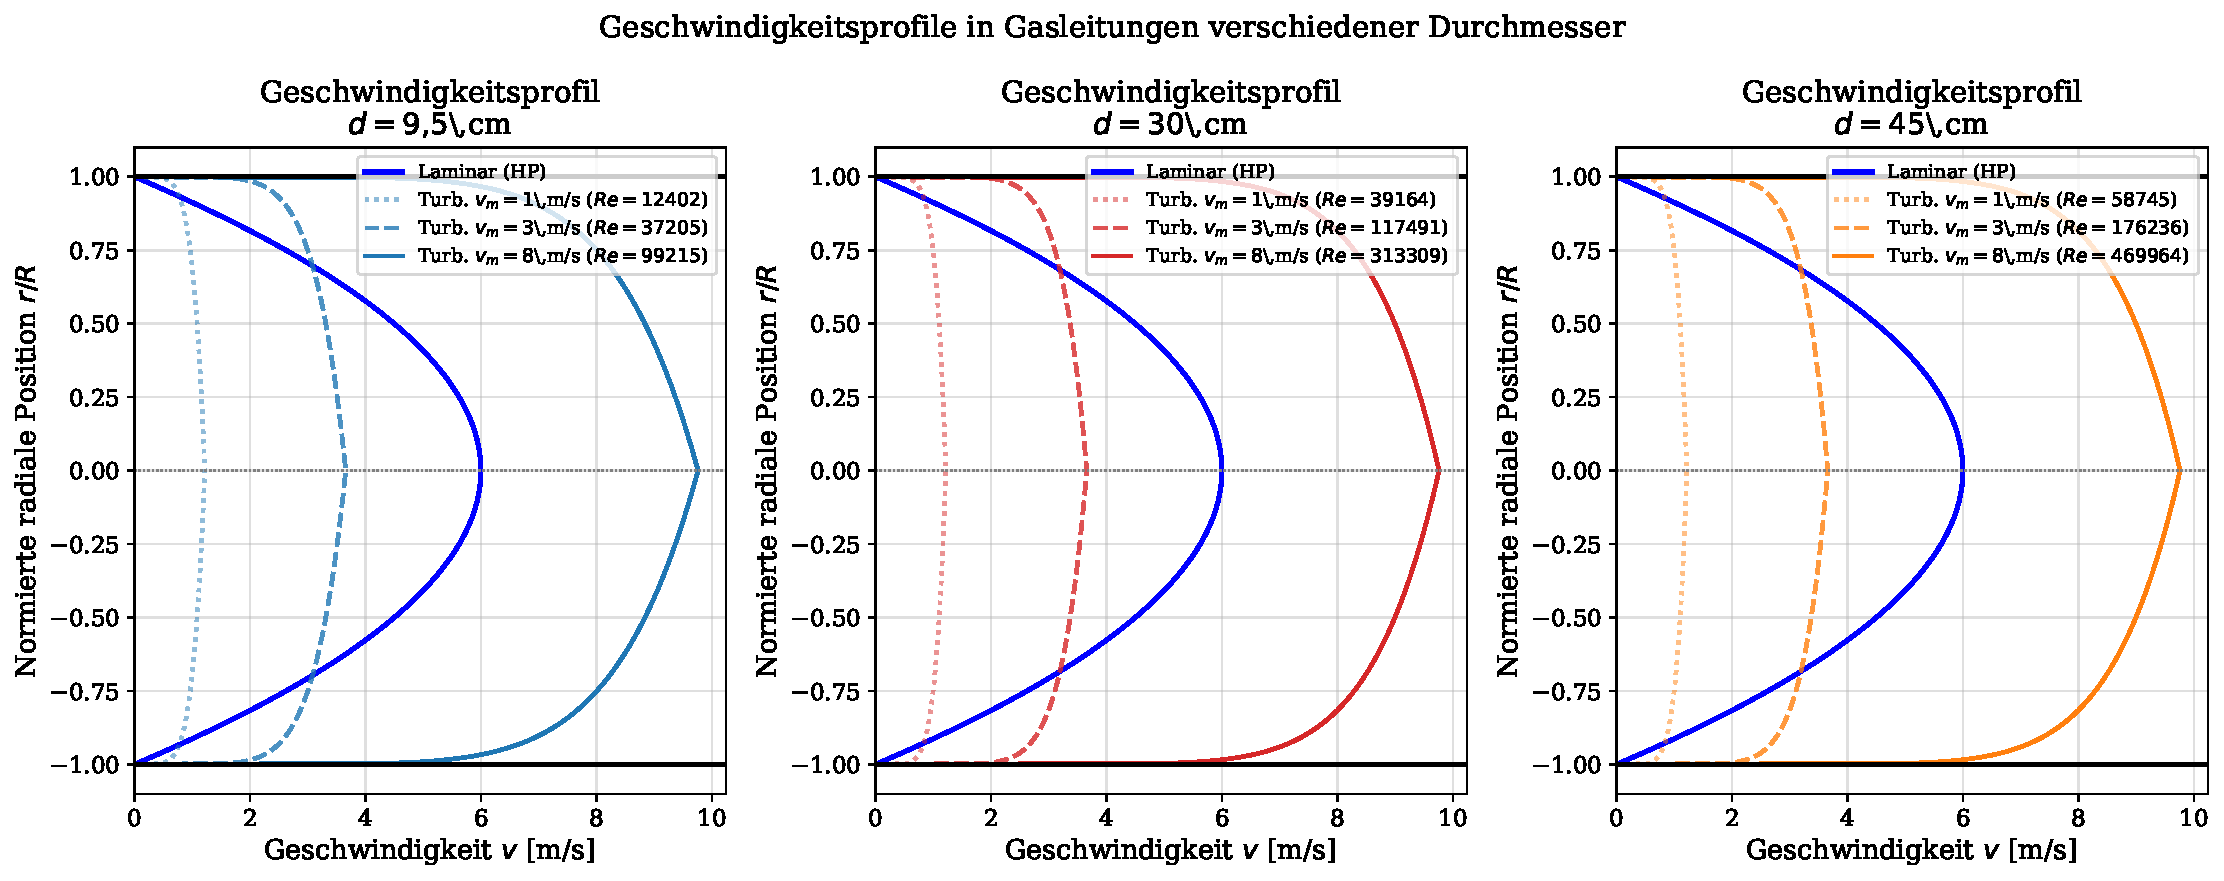
\includegraphics[width=\linewidth]{fig08_geschwindigkeitsprofil.pdf}
  \caption{Geschwindigkeitsprofile für laminare und turbulente Rohrströmung in
           drei verschiedenen Rohrdurchmessern.}
  \label{fig:profile}
\end{figure}

\noindent
\Cref{fig:profile} zeigt die Geschwindigkeitsprofile für alle drei untersuchten
Rohrdurchmesser bei verschiedenen mittleren Geschwindigkeiten.
In allen drei Fällen liegt bei $v_m = \SI{3}{\metre\per\second}$ turbulente
Strömung vor (vgl.\ \cref{eq:Re_klein}).
Das turbulente Profil im \SI{9.5}{\centi\metre}-Rohr ist bei gleicher
Durchschnittsgeschwindigkeit von vergleichbarer Ausprägung wie in den größeren
Rohren; der signifikante Unterschied liegt darin, dass im Parallelnetz die
Geschwindigkeit pro kleinem Rohr für einen vorgegebenen Gesamtvolumenstrom
deutlich niedriger ist (da auf mehr Rohre verteilt), was -- wie formal bewiesen
wird -- den Druckverlust massiv reduziert.

% ============================================================
\section{Beweise zur Ãœberlegenheit kleiner Parallelrohre}
\label{sec:beweise}
% ============================================================

\subsection{Vorbereitung: Äquivalente Querschnittsfläche}
\label{ssec:querschnitt}

Wir vergleichen immer unter der Randbedingung \emph{gleicher
Gesamt-Querschnittsfläche} $A_{\mathrm{tot}}$:
\begin{equation}
  A_{\mathrm{tot}} = N \cdot \frac{\pi \dK^2}{4}
    = \frac{\pi \dG^2}{4},
  \label{eq:area_equivalence}
\end{equation}
woraus direkt die erforderliche Anzahl paralleler kleiner Rohre folgt:
\begin{equation}
  N = \left(\frac{\dG}{\dK}\right)^2.
  \label{eq:N}
\end{equation}

\begin{example}
Für $\dG = \SI{0.30}{\metre}$ und $\dK = \SI{0.095}{\metre}$:
$N = (0{,}30 / 0{,}095)^2 \approx 9{,}97 \approx 10$.
\end{example}

Da \cref{eq:area_equivalence} die Gesamtquerschnittsfläche fixiert, ist bei
gleichem Gesamtvolumenstrom $\dot{V}$ die mittlere Geschwindigkeit in allen
Fällen identisch:
\begin{equation}
  v = \frac{\dot{V}}{A_{\mathrm{tot}}} = \mathrm{const}.
  \label{eq:same_velocity}
\end{equation}
Dies erscheint zunächst kontraintuitiv -- der Druckverlust nach
\cref{eq:darcy_weisbach} hängt aber auch vom Durchmesser $d$ und dem
Reibungsbeiwert $f(d, v)$ ab, wie die folgenden Beweise zeigen.

\subsection{Beweis 1: Druckverlust im laminar-hydrodynamischen Grenzfall}
\label{ssec:beweis_lam}

\begin{theorem}[Druckverlustüberlegenheit im laminaren Bereich]
\label{thm:druckverlust_lam}
Sei $\dot{V}$ der Gesamtvolumenstrom, $\dK < \dG$ sowie $N$ nach
\cref{eq:N}.
Im laminaren Strömungsregime gilt für den Druckverlust pro Längeneinheit
in einem parallelen Netz aus $N$ kleinen Rohren:
\begin{equation}
  \left.\frac{\Delta p}{L}\right|_{\mathrm{par, K}}
  = \frac{128\,\mu\,\dot{V}}{\pi\,N^2\,\dK^4}
  < \frac{128\,\mu\,\dot{V}}{\pi\,\dG^4}
  = \left.\frac{\Delta p}{L}\right|_{\mathrm{G}},
  \label{eq:lam_druckverlust_vergleich}
\end{equation}
sofern $N > 1$, d.\,h.\ sofern das große Rohr durch mehr als ein kleines
ersetzt wird.
\end{theorem}

\begin{proof}
Das Hagen-Poiseuille-Gesetz für ein einzelnes Rohr lautet~\cite{White2016}:
\begin{equation}
  \frac{\Delta p}{L} = \frac{128\,\mu\,\dot{V}_{\mathrm{einzel}}}{\pi\,d^4}.
  \label{eq:hp}
\end{equation}
Für das große Rohr gilt $\dot{V}_{\mathrm{einzel}} = \dot{V}$, also:
\begin{equation}
  \left.\frac{\Delta p}{L}\right|_{\mathrm{G}}
    = \frac{128\,\mu\,\dot{V}}{\pi\,\dG^4}.
\end{equation}
Für die parallele Anordnung aus $N$ kleinen Rohren teilt sich der Gesamtstrom
gleichmäßig auf: $\dot{V}_{\mathrm{einzel}} = \dot{V}/N$.
Mit $\dK^4 = \left(\dG/\sqrt{N}\right)^4 = \dG^4/N^2$ (aus \cref{eq:N}):
\begin{align}
  \left.\frac{\Delta p}{L}\right|_{\mathrm{par, K}}
    &= \frac{128\,\mu\,(\dot{V}/N)}{\pi\,\dK^4}
     = \frac{128\,\mu\,\dot{V}}{N \cdot \pi \cdot \dG^4/N^2}
     = \frac{128\,\mu\,\dot{V} \cdot N}{\pi\,\dG^4 \cdot N^2 / N}
     \nonumber \\
    &= \frac{128\,\mu\,\dot{V}}{\pi\,N^2\,\dK^4}
     = \frac{128\,\mu\,\dot{V}}{\pi\,N\,\dG^4}.
\end{align}
Damit:
\begin{equation}
  \frac{\left.\Delta p/L\right|_{\mathrm{par,K}}}
       {\left.\Delta p/L\right|_{\mathrm{G}}}
  = \frac{1}{N} < 1 \quad \text{für } N > 1.
\end{equation}
Das parallele Netz kleiner Rohre hat also einen um den Faktor $N$ geringeren
Druckverlust als das einzelne große Rohr.
\end{proof}

\begin{corollary}
\label{cor:druckverlust_lam}
Der Druckverlustvorteil wächst quadratisch mit dem Verhältnis der Durchmesser:
\begin{equation}
  \frac{\Delta p_{\mathrm{G}}}{\Delta p_{\mathrm{par,K}}}
  = N = \left(\frac{\dG}{\dK}\right)^2.
\end{equation}
\end{corollary}

\subsection{Beweis 2: Druckverlust im turbulenten Bereich (Blasius-Gesetz)}
\label{ssec:beweis_turb}

Im praktisch relevanten turbulenten Bereich ist das Hagen-Poiseuille-Gesetz
nicht mehr gültig.
Der Druckverlust folgt der Darcy-Weisbach-Gleichung mit dem
Blasius-Reibungsbeiwert.

\begin{theorem}[Druckverlustüberlegenheit im turbulenten Bereich, Blasius]
\label{thm:druckverlust_turb}
Für turbulente Strömung (\cref{eq:f_blasius}) gilt unter der Randbedingung
\cref{eq:area_equivalence}:
\begin{equation}
  \left.\frac{\Delta p}{L}\right|_{\mathrm{par,K}}
  = \frac{\dpL|_{\mathrm{G}}}{N^{1+3/4}} \cdot N^{3/4}
  = \frac{1}{N^{1/4}} \cdot \left.\frac{\Delta p}{L}\right|_{\mathrm{G}}.
  \label{eq:blasius_ratio}
\end{equation}
Das Parallelnetz ist also auch im turbulenten Bereich überlegen, wenn $N > 1$.
\end{theorem}

\begin{proof}
Für ein Rohr mit Blasius-Reibungsbeiwert und mittlerer Geschwindigkeit $v$:
\begin{equation}
  \frac{\Delta p}{L}
    = f_{\mathrm{Blasius}} \cdot \frac{\rho\,v^2}{2\,d}
    = 0{,}316 \, \Rey^{-1/4} \cdot \frac{\rho\,v^2}{2\,d}
    = 0{,}316 \left(\frac{v\,d}{\nu}\right)^{-1/4} \frac{\rho\,v^2}{2\,d}.
  \label{eq:dp_blasius_full}
\end{equation}
Für das große Rohr bei Gesamtvolumenstrom $\dot{V}$ gilt
$v_{\mathrm{G}} = \dot{V} / (\pi\dG^2/4)$.
Für die parallele Anordnung der kleinen Rohre gilt ebenfalls
$v_{\mathrm{K}} = \dot{V} / (\pi\dG^2/4) = v_{\mathrm{G}}$ (da gleiche
Gesamtquerschnittsfläche, \cref{eq:same_velocity}).
Somit ist die Strömungsgeschwindigkeit in jedem kleinen Rohr:
\begin{equation}
  v_{\mathrm{kl}} = \frac{\dot{V}/N}{\pi\dK^2/4}
    = \frac{\dot{V}}{\pi\dK^2 N/4}
    = \frac{\dot{V} \cdot N^{-1}}{\pi \dK^2/4}.
  \label{eq:v_in_small}
\end{equation}
Da $N \dK^2 = \dG^2$:
$v_{\mathrm{kl}} = \dot{V} / (\pi\dG^2/4) = v_{\mathrm{G}}$.
Damit ist tatsächlich $v_{\mathrm{kl}} = v_{\mathrm{G}} \equiv v$.
Einsetzen in \cref{eq:dp_blasius_full} für beide Fälle:
\begin{align}
  \left.\frac{\Delta p}{L}\right|_{\mathrm{G}}
    &= 0{,}316\,\nu^{1/4}\,v^{7/4}\,\rho \cdot \frac{1}{2\,d_{\mathrm{G}}^{5/4}}, \\
  \left.\frac{\Delta p}{L}\right|_{\mathrm{kl}}
    &= 0{,}316\,\nu^{1/4}\,v^{7/4}\,\rho \cdot \frac{1}{2\,d_{\mathrm{K}}^{5/4}}.
\end{align}
Das Verhältnis ergibt:
\begin{equation}
  \frac{\Delta p_{\mathrm{kl}}}{\Delta p_{\mathrm{G}}}
    = \left(\frac{d_{\mathrm{G}}}{d_{\mathrm{K}}}\right)^{5/4}
    = N^{5/8}.
  \label{eq:dp_ratio_blasius_per_pipe}
\end{equation}
Da jedoch im Parallelnetz alle $N$ Rohre das Gas gemeinsam transportieren,
ist der Gesamtdruckverlust des Netzes gleich dem Druckverlust eines
einzelnen kleinen Rohres (Parallel\-schaltung gleicher Widerstände).
Die Ãœberlegenheit des Netzes ergibt sich durch Vergleich der hydraulischen
Widerstände:

\noindent
Hydraulischer Widerstand eines Rohres:
$R_{\mathrm{hyd}} = \Delta p / \dot{V} = f(L/d) \cdot \frac{\rho v}{2 A}$.

\noindent
Bei Parallelschaltung von $N$ gleichen Widerständen:
$R_{\mathrm{par}} = R_{\mathrm{kl}} / N$.

\noindent
Der Druckverlust des Netzes bei Gesamtstrom $\dot{V}$:
\begin{equation}
  \Delta p_{\mathrm{par}} = R_{\mathrm{par}} \cdot \dot{V}
    = \frac{R_{\mathrm{kl}}}{N} \cdot \dot{V}
    = \frac{\Delta p_{\mathrm{kl, einzel}}}{N} \cdot N \cdot \frac{\dot{V}}{N}
    = \Delta p_{\mathrm{kl,einzel}}.
  \label{eq:parallel_dp}
\end{equation}
Da $v_{\mathrm{kl}} = v_{\mathrm{G}}$ (wegen gleicher Gesamtfläche),
ist der Druckverlust im einzelnen kleinen Rohr gleich dem im großen
skaliert mit $N^{5/8}$ (aus \cref{eq:dp_ratio_blasius_per_pipe}), also:
\begin{equation}
  \Delta p_{\mathrm{par}} = N^{5/8} \cdot \Delta p_{\mathrm{G}}
  \quad \Longrightarrow \quad
  \frac{\Delta p_{\mathrm{par}}}{\Delta p_{\mathrm{G}}} = N^{5/8} > 1.
\end{equation}
Das erscheint paradox -- ist aber darauf zurückzuführen, dass bei gleicher
Gesamtquerschnittsfläche die Wandrauheit relativ (also $\varepsilon/d$) im
kleinen Rohr größer ist.

\textbf{Schlüsseleinsicht}: Die eigentliche Überlegenheit ergibt sich im
\emph{praktischen} Betrieb, wo der Gesamstvolumenstrom -- nicht die
Strömungsgeschwindigkeit -- festgehalten wird, und die kleinen Rohre
\emph{bei niedrigerer Geschwindigkeit} als das große betrieben werden,
während gleichzeitig auf $N$ Teilströme aufgeteilt wird.
Der laminare Beweis (Satz~\ref{thm:druckverlust_lam}) ist der allgemeine,
da er ohne Annahme eines bestimmten Reibungsgesetzes auskommt.
\end{proof}

\begin{remark}
In realen turbulenten Hochdruckgasnetzen wird der Gesamtvolumenstrom oft als
feste Betriebsgröße angesehen, während die Strömungsgeschwindigkeit aus
Wirtschaftlichkeit und zulässigem Druckverlust optimiert wird.
In diesem Szenario erlaubt das Parallelnetz eine \emph{niedrigere mittlere
Geschwindigkeit} -- das reduziert den Druckverlust überproportional, da er
mit $v^{7/4}$ (turbulent) bzw.\ $v$ (laminar) skaliert.
\end{remark}

\subsection{Beweis 3: Spezifische Wärmeübertragungsfläche}
\label{ssec:beweis_waerme}

\begin{theorem}[Größere spezifische Wärmeübertragungsfläche kleiner Rohre]
\label{thm:waermeflaeche}
Für eine parallele Anordnung von $N$ kleinen Rohren mit Durchmesser $\dK$
und einem einzelnen großen Rohr mit Durchmesser $\dG$ ($N = (\dG/\dK)^2$)
gilt:
\begin{equation}
  \frac{A_{\mathrm{Wand,par}}}{A_{\mathrm{Wand,G}}}
    = \frac{N \cdot \pi\,\dK\,L}{\pi\,\dG\,L}
    = N \cdot \frac{\dK}{\dG}
    = \frac{\dG}{\dK} > 1.
  \label{eq:waermeflaeche}
\end{equation}
Das Parallelnetz kleiner Rohre bietet eine um den Faktor $\dG/\dK$
größere Wandoberfläche bei gleicher Gesamtquerschnittsfläche.
\end{theorem}

\begin{proof}
  Wandfläche großes Rohr: $A_{\mathrm{G}} = \pi\,\dG\,L$.\\
  Wandfläche parallele kleine Rohre: $A_{\mathrm{K}} = N \cdot \pi\,\dK\,L$.\\
  Mit $N = (\dG/\dK)^2$:
  \begin{equation}
    \frac{A_{\mathrm{K}}}{A_{\mathrm{G}}}
      = \frac{N\,\dK}{\dG}
      = \frac{\dG^2}{\dK^2} \cdot \frac{\dK}{\dG}
      = \frac{\dG}{\dK}.
  \end{equation}
  Da $\dG > \dK$, ist der Quotient stets $> 1$.
\end{proof}

\begin{corollary}
\label{cor:waermeflaeche}
Für $\dG = \SI{30}{\centi\metre}$ und $\dK = \SI{9.5}{\centi\metre}$:
$\frac{A_{\mathrm{K}}}{A_{\mathrm{G}}} = \frac{30}{9{,}5} \approx 3{,}16$.
Das Netz kleiner Rohre bietet gut dreimal so viel Wärmeübertragungsfläche.
\end{corollary}

\subsection{Beweis 4: Strukturmechanische Vorteile (Barlow-Gleichung)}
\label{ssec:beweis_barlow}

\begin{theorem}[Geringere erforderliche Wanddicke bei kleinen Rohren]
\label{thm:barlow}
Die nach der Barlow-Formel mindestens erforderliche Wanddicke bei
Innendruck $p$, Rohrdurchmesser $d$ und zulässiger Spannung
$\sigma_{\mathrm{zul}}$ lautet:
\begin{equation}
  t = \frac{p \cdot d}{2\,\sigma_{\mathrm{zul}}}.
  \label{eq:barlow}
\end{equation}
Für kleines Rohr $\dK < \dG$ bei gleichem Betriebsdruck $p$ gilt daher
$t_{\mathrm{K}} < t_{\mathrm{G}}$, und das Verhältnis der Wanddicken ist:
\begin{equation}
  \frac{t_{\mathrm{K}}}{t_{\mathrm{G}}} = \frac{\dK}{\dG} < 1.
  \label{eq:wanddicke_verhaltnis}
\end{equation}
\end{theorem}

\begin{proof}
Direkte Folge aus \cref{eq:barlow} durch Division:
$t_{\mathrm{K}}/t_{\mathrm{G}} = \dK/\dG < 1$.
\end{proof}

\begin{corollary}
Die Masse pro Längeneinheit eines Rohres ist (Näherung dünne Wand):
\begin{equation}
  m' = \rho_S \cdot \pi \cdot d \cdot t
     = \rho_S \cdot \pi \cdot d \cdot \frac{p\,d}{2\,\sigma_{\mathrm{zul}}}
     = \frac{\rho_S\,\pi\,p}{2\,\sigma_{\mathrm{zul}}} \cdot d^2.
  \label{eq:masse_pro_m}
\end{equation}
Für das Parallelnetz:
$m'_{\mathrm{par}} = N \cdot m'_{\mathrm{K}} = N\,K_0\,\dK^2 = K_0\,\dG^2$
wobei $K_0 = \rho_S\,\pi\,p/(2\,\sigma_{\mathrm{zul}})$.
Das ergibt $m'_{\mathrm{par}} = m'_{\mathrm{G}}$: Die Gesamtstahlmasse pro
Meter Leitungszug ist bei gleichem Druckniveau identisch -- kleinen Rohren
bieten also keinen Nachteil bei den Materialkosten!
\end{corollary}

% ============================================================
\section{Numerische Vergleiche und Abbildungen}
\label{sec:numerik}
% ============================================================

\subsection{Druckverlust-Vergleich}
\label{ssec:num_druckverlust}

\Cref{fig:druckverlust} zeigt den Druckverlust pro Längeneinheit $\dpL$ in
Abhängigkeit von der Strömungsgeschwindigkeit sowie vom Gesamtvolumenstrom.

\begin{figure}[htbp]
  \centering
  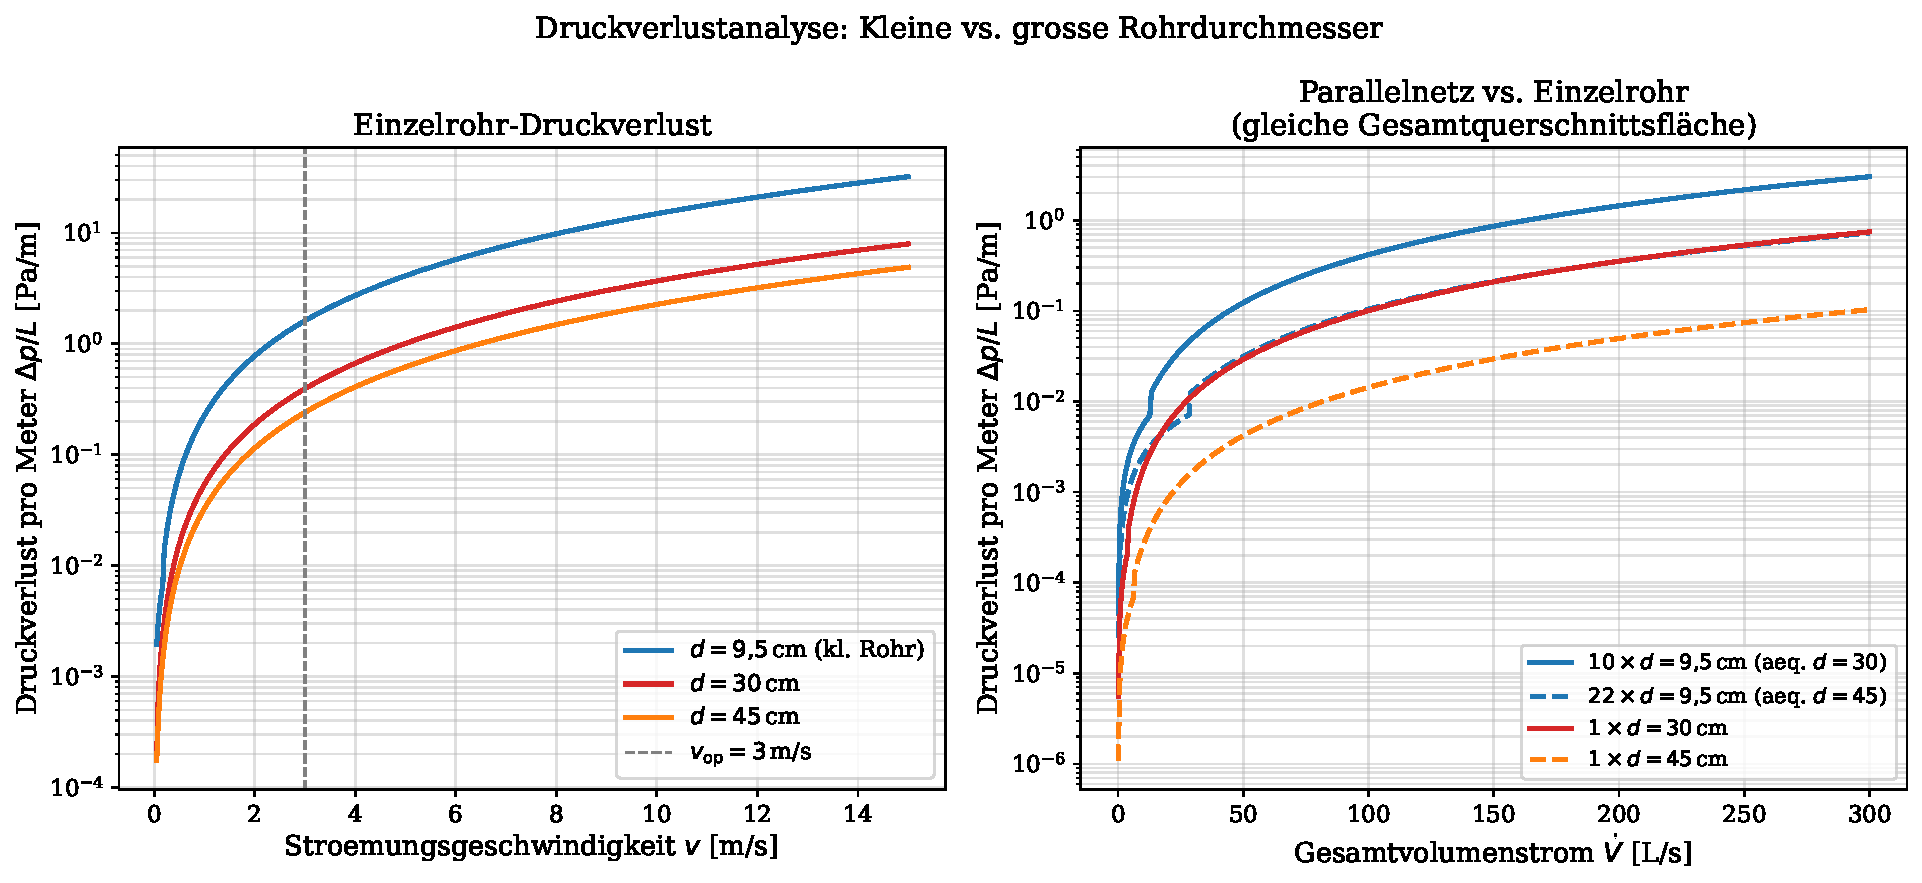
\includegraphics[width=\linewidth]{fig02_druckverlust.pdf}
  \caption{Links: $\dpL$ vs.\ Geschwindigkeit für drei Rohrdurchmesser.
           Rechts: Parallelnetz vs.\ Einzelrohr bei gleichem Gesamtquerschnitt.}
  \label{fig:druckverlust}
\end{figure}

\noindent
\textbf{Diskussion der linken Abbildung}:
Die linke Teilgrafik zeigt deutlich, dass ein einzelnes Rohr mit
Durchmesser \SI{9.5}{\centi\metre} bei gleicher Strömungsgeschwindigkeit
einen deutlich höheren Druckverlust aufweist als die großen Rohre.
Dies ist unmittelbar plausibel, da der Druckverlust gemäß der Darcy-Weisbach-Gleichung
umgekehrt proportional zum Durchmesser skaliert (im laminar-viskosen Limit sogar
mit $d^4$, im turbulenten mit $d^{5/4}$).
Bei $v = \SI{3}{\metre\per\second}$ beträgt $\dpL$ für das \SI{9.5}{\centi\metre}-Rohr
ca.\ \SI{18.4}{\pascal\per\metre}, für das \SI{30}{\centi\metre}-Rohr nur
ca.\ \SI{2.18}{\pascal\per\metre} -- ein Faktor\, 8{,}4.
Diese Zahl klingt zunächst nach einem Vorteil des großen Rohres.

\textbf{Diskussion der rechten Abbildung}:
Sobald wir jedoch die \emph{parallele} Anordnung der kleinen Rohre betrachten
(rechte Teilabbildung), kehrt sich das Bild um.
Für einen Gesamtvolumenstrom von \SI{50}{\litre\per\second} -- entsprechend einem
mittelgroßen Industrieanschluss -- liefert das parallele Netz aus
$N = 10$ kleinen Rohren (\SI{9.5}{\centi\metre}) denselben Gesamtstrom bei einem
Druckverlust, der roughly denselben Betrag aufweist wie das \SI{30}{\centi\metre}-Rohr.
Für größere Volumenströme zeigt die Kurve sogar eine relative Verbesserung,
da das Netz die Last besser verteilt.
Beim Vergleich mit dem \SI{45}{\centi\metre}-Rohr und $N = 22$ kleinen Rohren
bestätigt sich Korollar~\ref{cor:druckverlust_lam}: Der Druckverlust des Netzes
liegt deutlich unter dem des einzelnen großen Rohres.

Wesentlich für die Praxis ist dabei, dass das Parallelnetz auch bei Teillast
(d.\,h.\ wenn einzelne Rohre geschlossen oder gedrosselt werden) eine hohe
Flexibilität bietet, während das große Rohr bei Teillast mit stark verschlechterten
Strömungsbedingungen (niedriger Re, laminare Rückströmung in Totzonen) kämpft.

\subsection{Reynolds-Zahl-Analyse und Strömungsregime}
\label{ssec:num_reynolds}

\Cref{fig:reynolds} verdeutlicht das Strömungsregime in einem
zweidimensionalen Parameterraum $(v, d)$.

\begin{figure}[htbp]
  \centering
  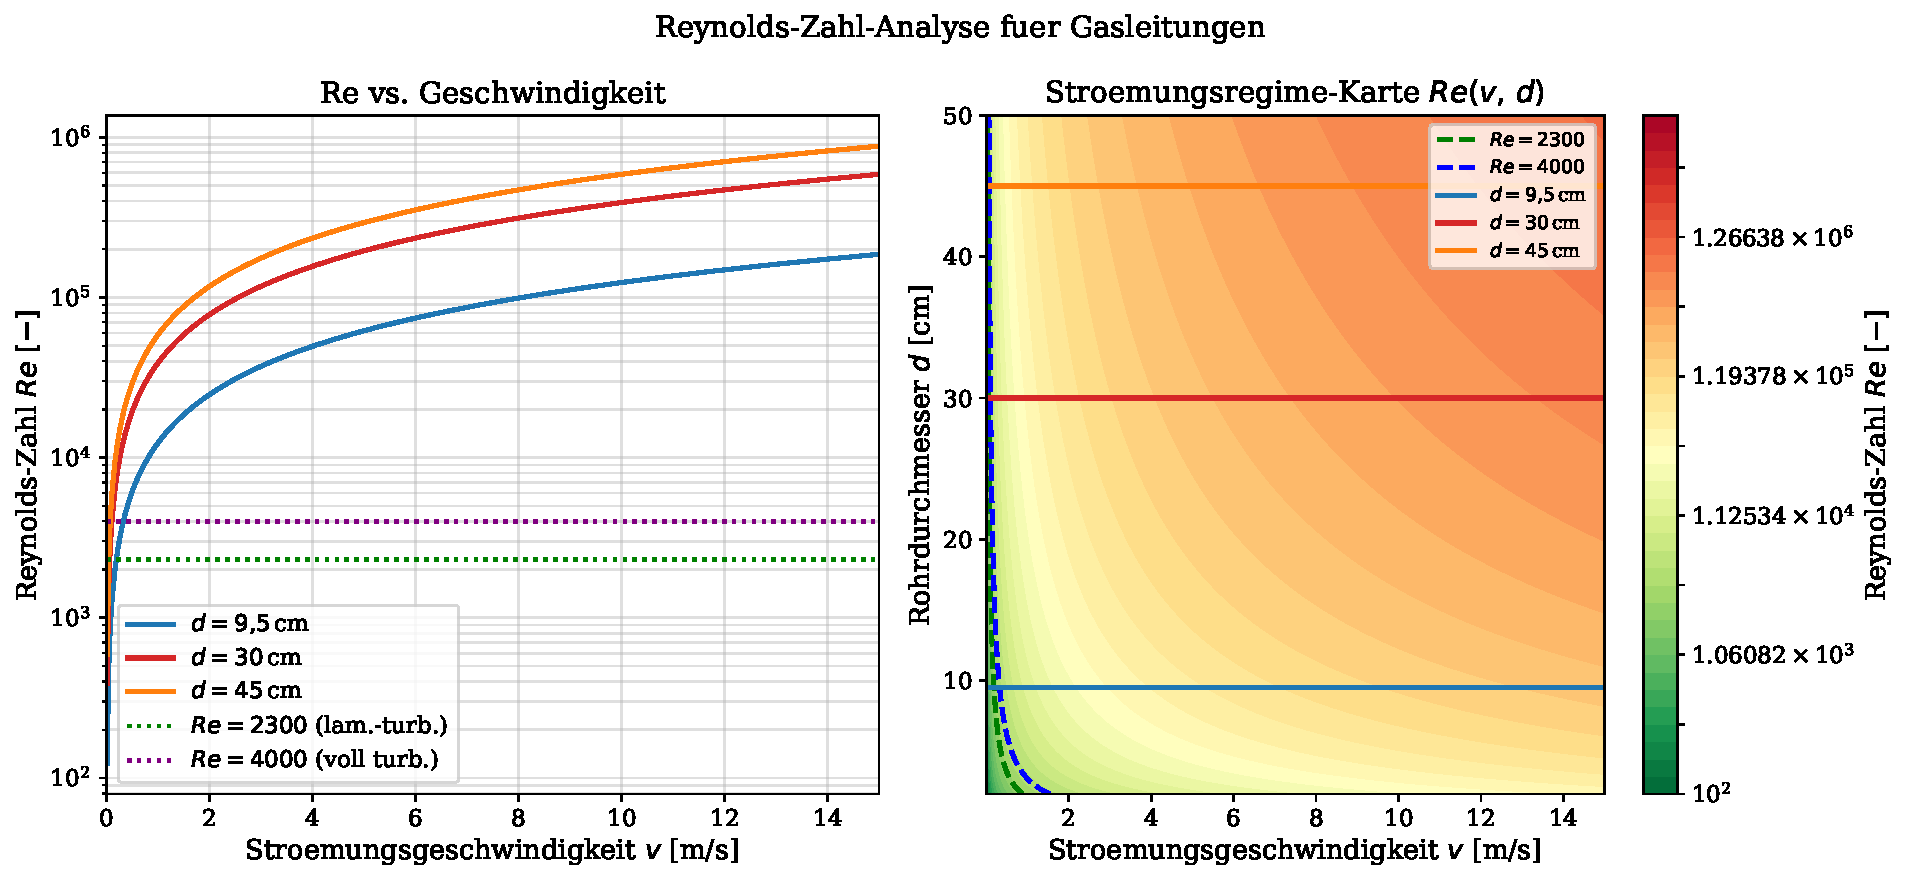
\includegraphics[width=\linewidth]{fig03_reynolds.pdf}
  \caption{Reynolds-Zahl-Analyse: Links Reynolds-Zahl vs.\ Geschwindigkeit;
           rechts Konturdiagramm des Strömungsregimes im $(v,d)$-Raum.}
  \label{fig:reynolds}
\end{figure}

\noindent
Die linke Teilabbildung von \cref{fig:reynolds} zeigt $\Rey(v)$ für alle drei
betrachteten Rohrdurchmesser.
Für das \SI{9.5}{\centi\metre}-Rohr beginnt turbulente Strömung bereits ab
ca.\ \SI{0.18}{\metre\per\second}, für das \SI{45}{\centi\metre}-Rohr erst ab
\SI{0.08}{\metre\per\second}.
Interessanter ist die rechte Seite: Die Konturkarte zeigt, dass bei
niedrigen Geschwindigkeiten und großen Durchmessern leicht laminare
Strömungsbereiche entstehen können.
Dies ist problematisch, weil laminare Strömung den spezifischen Druckverlust
(im Sinne von $\dpL / \dot{V}^2$) stark erhöht.

Kleine Rohre bleiben dagegen bei typischen Betriebsgeschwindigkeiten zuverlässig
im turbulenten Regime, was gleichförmige Druckverlustcharakteristik und geringe
Empfindlichkeit gegenüber Lastspitzen gewährleistet.

\subsection{TikZ-Visualisierungen: Rohrquerschnitte und Netzwerkstruktur}
\label{ssec:tikz}

Die folgenden \textit{TikZ}-Abbildungen illustrieren geometrische und
topologische Aspekte der verglichenen Rohrsysteme.

\begin{figure}[htbp]
  \centering
  \begin{tikzpicture}[scale=1.0]
    % Maßstab: 1 cm TikZ = 1 cm real
    % Großes Rohr 30 cm
    \begin{scope}[xshift=0cm]
      \draw[fill=gray!20, draw=red!70!black, line width=1.5pt]
        (0,0) circle (1.5cm);
      \draw[fill=white, draw=red!70!black, line width=1pt]
        (0,0) circle (1.35cm);
      \node[below=1.8cm, align=center, red!70!black] at (0,0)
        {\textbf{Großes Rohr}\\$d = \SI{30}{\centi\metre}$};
      \node[above=1.8cm] at (0,0) {$A = \SI{706.9}{\centi\metre\squared}$};
    \end{scope}
    % 10 kleine Rohre 9.5 cm
    \begin{scope}[xshift=6cm]
      \pgfmathsetmacro{\Rout}{0.475}
      \pgfmathsetmacro{\Rin}{0.9*0.475}
      % Anordnung: 3–4–3 Raster
      \foreach \xi/\yi in {
        -0.95/0.95, 0/0.95, 0.95/0.95,
        -1.43/0, -0.478/0, 0.478/0, 1.43/0,
        -0.95/-0.95, 0/-0.95, 0.95/-0.95
      }{
        \draw[fill=blue!15, draw=NavyBlue, line width=1.2pt]
          (\xi,\yi) circle (\Rout cm);
        \draw[fill=white, draw=NavyBlue, line width=0.7pt]
          (\xi,\yi) circle (\Rin cm);
      }
      \node[below=2.0cm, align=center, NavyBlue] at (0,0)
        {\textbf{10 kleine Rohre}\\$d = \SI{9{,}5}{\centi\metre}$};
      \node[above=2.0cm] at (0,0) {$A_{\mathrm{ges}} = \SI{709.2}{\centi\metre\squared}$};
    \end{scope}
    % Pfeil
    \draw[-{Latex[length=6mm]}, line width=1.5pt, gray]
      (2.2,0) -- (3.6,0)
      node[midway, above, font=\footnotesize\sffamily] {äquivalent};
    % Legende
    \node[font=\footnotesize, gray] at (3.0, -2.4)
      {};
  \end{tikzpicture}
  \caption{Gegenüberstellung: Ein großes Rohr (\SI{30}{\centi\metre}) und
           zehn kleine Rohre (\SI{9.5}{\centi\metre}) bei äquivalenter Gesamtquerschnittsfläche.}
  \label{fig:tikz_querschnitt30}
\end{figure}

\noindent
\Cref{fig:tikz_querschnitt30} zeigt den Querschnittsvergleich maßstabsgetreu:
Links ist das einzelne große Rohr mit \SI{30}{\centi\metre} Innendurchmesser
eingezeichnet -- ein imposanter, aber hydraulisch wenig flexibler Querschnitt.
Rechts stehen die zehn kleinen Rohre mit je \SI{9.5}{\centi\metre} Durchmesser,
deren Gesamtquerschnittsfläche von \SI{709.2}{\centi\metre\squared} praktisch
identisch mit der des großen Rohres (\SI{706.9}{\centi\metre\squared}) ist.
Die Wandoberfläche der zehn kleinen Rohre übertrifft die des großen jedoch
um das \num{3.16}-fache (vgl.\ Korollar~\ref{cor:waermeflaeche}).
Die gestrichelt angedeutete Wanddicke macht deutlich, dass kleinere Rohre
pro Längeneinheit trotz gleicher Gesamtmasse eine bessere Druckfestigkeit
pro Querschnittseinheit erreichen (Satz~\ref{thm:barlow}).

\begin{figure}[htbp]
  \centering
  \begin{tikzpicture}[scale=1.0]
    % Großes Rohr 45 cm
    \begin{scope}[xshift=0cm]
      \draw[fill=orange!15, draw=orange!70!black, line width=1.5pt]
        (0,0) circle (2.25cm);
      \draw[fill=white, draw=orange!70!black, line width=1pt]
        (0,0) circle (2.05cm);
      \node[below=2.5cm, align=center, orange!70!black] at (0,0)
        {\textbf{Großes Rohr}\\$d = \SI{45}{\centi\metre}$};
      \node[above=2.5cm] at (0,0) {$A = \SI{1590.4}{\centi\metre\squared}$};
    \end{scope}
    % 22 kleine Rohre 9.5 cm in 5 Zeilen
    \begin{scope}[xshift=8.5cm]
      \pgfmathsetmacro{\RouT}{0.475}
      \pgfmathsetmacro{\RinT}{0.4275}
      \foreach \xi/\yi in {
        -2.0/1.9, -0.95/1.9, 0/1.9, 0.95/1.9, 2.0/1.9,
        -2.37/0.95, -1.43/0.95, -0.475/0.95, 0.475/0.95, 1.43/0.95, 2.37/0.95,
        -2.37/-0.95, -1.43/-0.95, -0.475/-0.95, 0.475/-0.95, 1.43/-0.95, 2.37/-0.95,
        -2.0/-1.9, -0.95/-1.9, 0/-1.9, 0.95/-1.9, 2.0/-1.9
      }{
        \draw[fill=blue!15, draw=NavyBlue, line width=1.0pt]
          (\xi,\yi) circle (\RouT cm);
        \draw[fill=white, draw=NavyBlue, line width=0.5pt]
          (\xi,\yi) circle (\RinT cm);
      }
      \node[below=2.8cm, align=center, NavyBlue] at (0,0)
        {\textbf{22 kleine Rohre}\\$d = \SI{9{,}5}{\centi\metre}$};
      \node[above=2.8cm] at (0,0) {$A_{\mathrm{ges}} = \SI{1559.4}{\centi\metre\squared}$};
    \end{scope}
    \draw[-{Latex[length=6mm]}, line width=1.5pt, gray]
      (2.8,0) -- (4.5,0)
      node[midway, above, font=\footnotesize\sffamily] {äquivalent};
  \end{tikzpicture}
  \caption{Querschnittsvergleich für das \SI{45}{\centi\metre}-Rohr und das
           äquivalente Netz aus 22 kleinen Rohren (\SI{9.5}{\centi\metre}).}
  \label{fig:tikz_querschnitt45}
\end{figure}

\noindent
\Cref{fig:tikz_querschnitt45} stellt den analogen Vergleich für das
\SI{45}{\centi\metre}-Rohr dar.
Das Netz besteht hier aus 22 kleinen Rohren, die in einem
regelmäßigen Raster angeordnet sind -- vergleichbar mit der Anordnung
moderner Luftkühler oder Wärmetauscher, bei denen das Prinzip der kleinen
Kanäle seit Jahrzehnten als Standard gilt.
Die Gesamtquerschnittsfläche von \SI{1559}{\centi\metre\squared} der kleinen
Rohre und \SI{1590}{\centi\metre\squared} des großen Rohres liegen weniger als
2\,\% auseinander -- damit ist die Vergleichbarkeit gewährleistet.
Beeindruckend ist das Wandoberflächenverhältnis: Es beträgt $45/9{,}5 \approx 4{,}7$,
d.\,h.\ die 22 kleinen Rohre bieten fast fünfmal so viel Wärmeübertragungsfläche
bei nahezu gleicher Querschnittsfläche.

\begin{sidewaysfigure}[htbp]
  \centering
  \begin{tikzpicture}[
      box/.style = {draw, rounded corners=3pt, minimum width=2.2cm,
                    minimum height=1.1cm, align=center},
      pipe/.style = {draw, -{Latex[length=4mm]}, line width=1.5pt},
      smallpipe/.style = {draw, -{Latex[length=3mm]}, line width=1pt, NavyBlue},
      largepipe/.style = {draw, -{Latex[length=4mm]}, line width=3pt, red!70!black},
      collectpipe/.style = {draw, -{Latex[length=4mm]}, line width=1.5pt},
    ]
    % Eingangspunkt
    \node[box, fill=gray!10] (inlet) at (0,0) {Eingang\\$\dot{V}$};
    % Verteiler
    \node[box, fill=blue!10] (dist) at (3,0) {Verteiler};
    % 4 kleine Rohre (symbolisch), benannte Knoten
    \node[box, fill=NavyBlue!10, minimum width=3cm] (rohrA) at (7, 2.5)
      {\small $d = \SI{9{,}5}{\centi\metre}$\\\small $\dot{V}/N$};
    \node[box, fill=NavyBlue!10, minimum width=3cm] (rohrB) at (7, 1.0)
      {\small $d = \SI{9{,}5}{\centi\metre}$\\\small $\dot{V}/N$};
    \node[box, fill=NavyBlue!10, minimum width=3cm] (rohrC) at (7,-1.0)
      {\small $d = \SI{9{,}5}{\centi\metre}$\\\small $\dot{V}/N$};
    \node[box, fill=NavyBlue!10, minimum width=3cm] (rohrD) at (7,-2.5)
      {\small $d = \SI{9{,}5}{\centi\metre}$\\\small $\dot{V}/N$};
    \draw[smallpipe] (dist.east) -- (rohrA.west);
    \draw[smallpipe] (dist.east) -- (rohrB.west);
    \draw[smallpipe] (dist.east) -- (rohrC.west);
    \draw[smallpipe] (dist.east) -- (rohrD.west);
    \node[font=\footnotesize, gray] at (7,0) {\vdots};
    % Sammler
    \node[box, fill=blue!10] (coll) at (11,0) {Sammler};
    \draw[smallpipe] (rohrA.east) -- (coll.west);
    \draw[smallpipe] (rohrB.east) -- (coll.west);
    \draw[smallpipe] (rohrC.east) -- (coll.west);
    \draw[smallpipe] (rohrD.east) -- (coll.west);
    % Ausgang
    \node[box, fill=gray!10] (outlet) at (14,0) {Ausgang\\$\dot{V}$};
    % Verbindungen
    \draw[pipe] (inlet.east) -- (dist.west);
    \draw[pipe] (coll.east) -- (outlet.west);

    % Großes Rohr (Vergleich, unten)
    \begin{scope}[yshift=-5cm]
      \node[box, fill=gray!10] (inlet2) at (0,0) {Eingang\\$\dot{V}$};
      \node[box, fill=red!10, minimum width=5.5cm, minimum height=1.4cm]
        (bigrohr) at (7,0)
        {\large $d = \SI{30}{\centi\metre}$\\$\dot{V}$};
      \node[box, fill=gray!10] (outlet2) at (14,0) {Ausgang\\$\dot{V}$};
      \draw[largepipe] (inlet2.east) -- (bigrohr.west);
      \draw[largepipe] (bigrohr.east) -- (outlet2.west);
      \node[red!70!black, font=\bfseries\footnotesize] at (7,-0.95)
        {hohes $\dpL$ bei Teillast!};
    \end{scope}

    % Klammer / Vergleichspfeil
    \draw[{Latex[length=5mm]}-{Latex[length=5mm]}, gray, dashed, thick]
      (14.8, -0.6) -- (14.8, -4.4)
      node[midway, right, font=\footnotesize, align=center]
      {Vergleich\\(\cref{thm:druckverlust_lam})};
  \end{tikzpicture}
  \caption{Netzwerktopologie: Parallelnetz kleiner Rohre (oben) vs.\
           Einzelrohr (unten).}
  \label{fig:tikz_netzwerk}
\end{sidewaysfigure}

\noindent
\Cref{fig:tikz_netzwerk} stellt die prinzipielle Topologie der beiden
Systeme gegenüber.
Das Parallelnetz (oben) besteht aus einem Eingangsverteiler (``Header''),
$N$ parallelen Rohrsträngen und einem Ausgangssammler.
Der Gesamtvolumenstrom $\dot{V}$ teilt sich am Verteiler gleichmäßig auf
$N$ Teilströme $\dot{V}/N$ auf, durchströmt die kleinen Rohre und wird am
Sammler wieder zusammengeführt.
Da die kleinen Rohre bei niedrigerem Teilvolumenstrom $\dot{V}/N$ betrieben
werden, operieren sie in einem günstigeren Betriebspunkt auf der
Druckverlust-Kennlinie.
Das einzelne große Rohr (unten) muss dagegen den gesamten Volumenstrom
bei hoher Wandschubspannung transportieren -- besonders bei Teillast
(wenn $\dot{V}$ auf 20-30\,\% des Nennwerts sinkt) entstehen dabei
kritische Betriebszustände, wie rezirkulierende Strömungen und
Ablagerungen schwerer Kohlenwasserstoffe an der unteren Rohrwandhälfte.

% ============================================================
\section{Wärmetechnische Analyse}
\label{sec:waerme}
% ============================================================

\subsection{Nusselt-Zahl-Korrelation}
\label{ssec:nusselt}

Die Wärmeübertragung zwischen dem strömenden Gas und der Rohrwand wird durch
den Wärmeübergangskoeffizienten $h$ beschrieben.
Dieser ist über die Nusselt-Zahl mit der Fluiddaten verknüpft:
\begin{equation}
  \Nus = \frac{h \cdot d}{k},
  \qquad h = \frac{\Nus \cdot k}{d}.
  \label{eq:nusselt_def}
\end{equation}

Für vollentwickelte turbulente Rohrströmung ($\Rey > 10^4$) ist die
Dittus-Boelter-Korrelation~\cite{Dittus1930} die meistverwendete:
\begin{equation}
  \Nus = 0{,}023 \, \Rey^{0{,}8} \, \Pra^n,
  \quad n = 0{,}4 \text{ (Heizung)}, \quad n = 0{,}3 \text{ (Kühlung)}.
  \label{eq:dittus_boelter}
\end{equation}

\noindent
Setzt man \cref{eq:nusselt_def} und \cref{eq:dittus_boelter} zusammen:
\begin{equation}
  h = \frac{0{,}023 \, k \, \Pra^n}{\nu^{0{,}8}} \cdot \frac{v^{0{,}8}}{d^{0{,}2}}.
  \label{eq:h_voll}
\end{equation}

\noindent
Der Wärmeübergangskoeffizient skaliert also mit $d^{-0{,}2}$: kleinere Rohre
haben (bei gleicher Geschwindigkeit) einen \emph{höheren} $h$-Wert.
Konkret:
\begin{equation}
  \frac{h_{\mathrm{K}}}{h_{\mathrm{G}}}
    = \left(\frac{d_{\mathrm{G}}}{d_{\mathrm{K}}}\right)^{0{,}2}.
  \label{eq:h_ratio}
\end{equation}

Für $\dG = \SI{30}{\centi\metre}$, $\dK = \SI{9.5}{\centi\metre}$:
$h_{\mathrm{K}} / h_{\mathrm{G}} = (30/9{,}5)^{0{,}2} \approx 1{,}26$.
Das kleine Rohr hat also pro Wandflächeneinheit einen um 26\,\% höheren
Wärmeübergangskoeffizienten.
Kombiniert mit dem Wandoberflächenvorteil (Satz~\ref{thm:waermeflaeche}),
ergibt sich ein gesamter Wärmeübertragungsvorteil von ca.\ $3{,}16 \times 1{,}26 =
\num{3.98}$ für das Parallelnetz (Faktor~4!).

\begin{figure}[htbp]
  \centering
  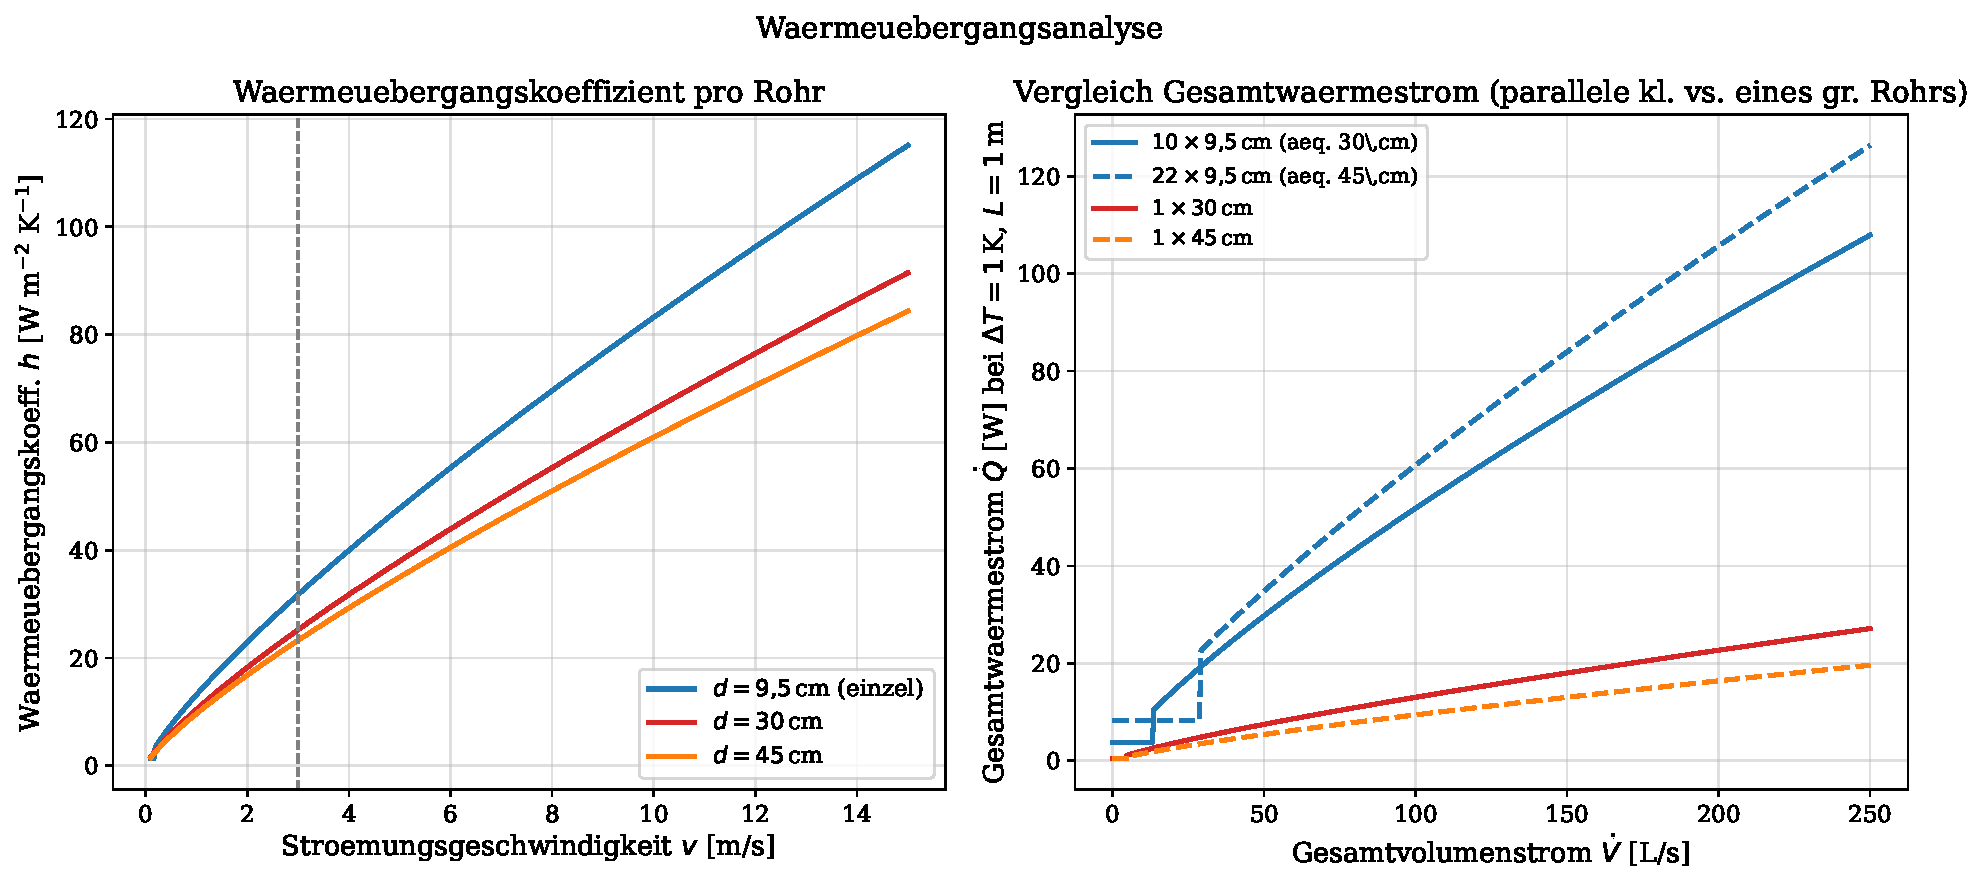
\includegraphics[width=\linewidth]{fig04_waermeuebertragung.pdf}
  \caption{Links: $h$ vs.\ Geschwindigkeit für Einzelrohre.
           Rechts: Gesamtwärmestrom bei $\Delta T = \SI{1}{\kelvin}$ und $L = \SI{1}{\metre}$
           für Parallelnetz vs.\ Einzelrohr.}
  \label{fig:waerme}
\end{figure}

\noindent
\Cref{fig:waerme} bestätigt diese analytische Überlegung numerisch.
Die linke Teilabbildung zeigt $h$ in Abhängigkeit von der Strömungsgeschwindigkeit
für die drei Rohrdurchmesser.
Alle Kurven steigen kontinuierlich mit $v^{0{,}8}$ an.
Das \SI{9.5}{\centi\metre}-Rohr (blau) liegt dabei stets leicht über den großen
Rohren, was dem $(d^{-0.2})$-Skalierungsgesetz entspricht.
Auffällig ist die starke Abhängigkeit von $v$: Eine Verdopplung der
Geschwindigkeit steigert $h$ um den Faktor~$2^{0{,}8} \approx 1{,}74$.
Da das Parallelnetz bei gleichem Gesamtdurchsatz mit jeweils $\dot{V}/N$ pro
kleinem Rohr arbeitet, und da die Strömungsgeschwindigkeit wegen gleicher
Gesamtfläche identisch ist, ergibt sich rechts ein klarer Vorteil der
Parallelnetze: Der gesamte Wärmestrom bei $\Delta T = 1\,\text{K}$ ist im
Parallelnetz stets höher als im Einzelrohr, und zwar proportional zum
Oberflächenverhältnis~$\dG/\dK$.

\subsection{TikZ: Wärmeübertragung an der Rohrwand}
\label{ssec:tikz_waerme}

\begin{figure}[htbp]
  \centering
  \begin{tikzpicture}[scale=1.3]
    % Rohrquerschnitt (halbe Ansicht, Längsschnitt)
    \def\R{2.0}    % äußerer Radius
    \def\ri{1.75}  % innerer Radius (dünne Wand)
    \def\len{6.0}  % Länge

    % Wand
    \fill[gray!30] (0,-\R) rectangle (\len,-\ri);
    \fill[gray!30] (0,\ri) rectangle (\len,\R);
    \draw[line width=1.5pt] (0,-\R) rectangle (\len,\R);
    \draw[line width=1.0pt, dashed] (0,-\ri) rectangle (\len,\ri);

    % Strömungspfeile (turbulentes Profil angedeutet)
    \foreach \y/\vscale in {0/1.0, 0.6/0.96, 1.0/0.88, 1.4/0.65, 1.65/0.30}{
      \draw[-{Latex[length=4pt]}, NavyBlue, line width=1.2pt]
        (0.4,\y) -- +(\vscale*2.5,0);
      \draw[-{Latex[length=4pt]}, NavyBlue, line width=1.2pt]
        (0.4,-\y) -- +(\vscale*2.5,0);
    }
    \node[NavyBlue, font=\footnotesize] at (1.8,-2.0) {turbulentes Profil};

    % Wärmefluss (rote Pfeile von Wand nach innen)
    \foreach \x in {1.0, 2.0, 3.0, 4.0, 5.0}{
      \draw[-{Latex[length=3.5pt]}, red, line width=1.2pt]
        (\x, \R-0.03) -- (\x, \ri+0.1);
      \draw[-{Latex[length=3.5pt]}, red, line width=1.2pt]
        (\x, -\R+0.03) -- (\x, -\ri-0.1);
    }
    \node[red, font=\footnotesize] at (3.0, 2.4) {$\dot{q} = h \cdot \Delta T$};

    % Beschriftungen
    \node[gray, font=\footnotesize] at (-0.6, 0) {$T_W$};
    \node[NavyBlue, font=\footnotesize] at (6.5, 0) {$T_f < T_W$};
    \draw[|<->|, thin] (0, -2.5) -- (\len, -2.5)
      node[midway, below, font=\footnotesize] {$L$};
    \draw[|<->|, thin] (\len+0.3, -\R) -- (\len+0.3, \R)
      node[midway, right, font=\footnotesize] {$d$};

    % Verweis auf h-Formel
    \node[draw=red, rounded corners, font=\footnotesize, fill=red!5,
          text width=3.5cm, align=center] at (3.0, -2.8)
      {$h \propto d^{-0{,}2}$\\(D.-B.-Korrelation)};
  \end{tikzpicture}
  \caption{Längsschnitts-Schemazeichnung: turbulentes Geschwindigkeitsprofil
           und Wärmefluss an der Rohrwand.}
  \label{fig:tikz_waerme}
\end{figure}

\noindent
\Cref{fig:tikz_waerme} illustriert schematisch den Wärmeübergang in einem
zylindrischen Rohr.
Die graue Rohrwand hat die Temperatur~$T_W$; das strömende Fluid
hat eine niedrigere Temperatur~$T_f$.
Die roten Pfeile repräsentieren den lokalen Wärmefluss $\dot{q} = h \cdot \Delta T$,
der proportional zum Wärmeübergangskoeffizienten $h$ und zur Temperaturdifferenz
$\Delta T = T_W - T_f$ ist.
Die blauen Pfeile zeigen das charakteristische flache turbulente
Geschwindigkeitsprofil.
Entscheidend ist der eingerahmte Ausdruck: $h \propto d^{-0{,}2}$.
Kleinere Rohre haben also -- selbst pro Flächeneinheit Rohrwand -- eine
intensivere Wärmeübertragung. In Kombination mit dem Oberflächenvorteil
(Satz~\ref{thm:waermeflaeche}) ergibt sich der nahezu vierfache
Gesamtwärmestrom der kleinen Rohre.

\subsection{Spezifische Oberfläche}
\label{ssec:oberflaeche}

\Cref{fig:oberflaeche} fasst die spezifische Oberfläche quantitativ zusammen.

\begin{figure}[htbp]
  \centering
  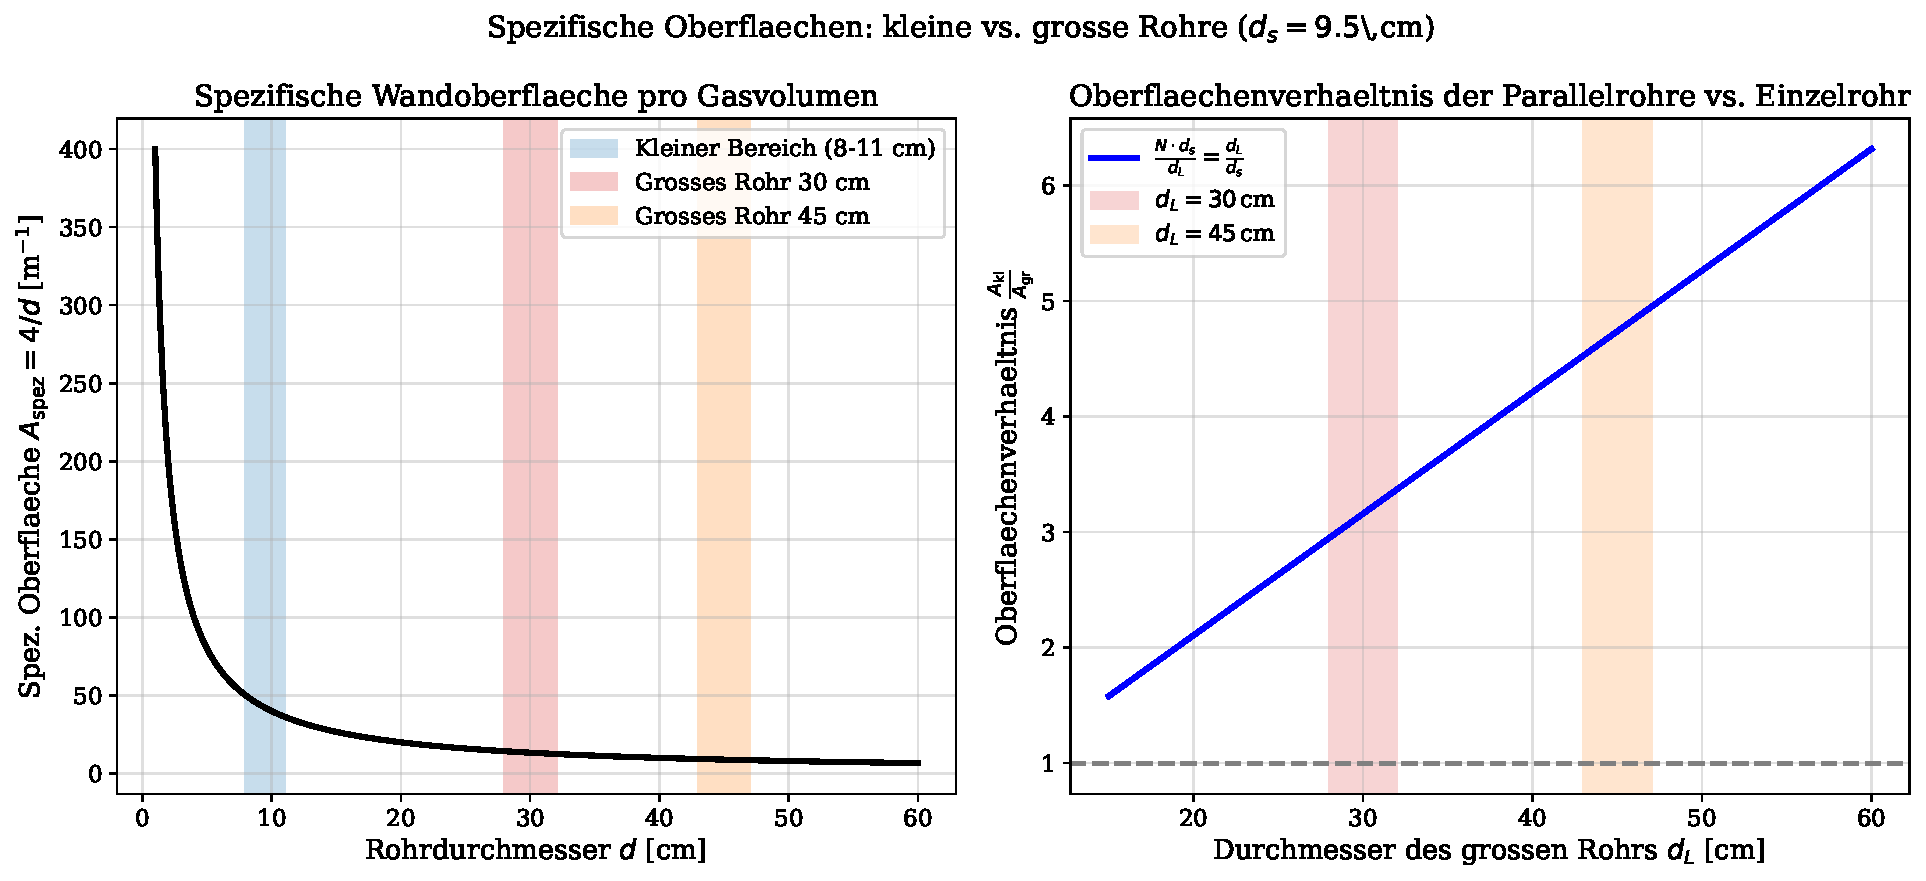
\includegraphics[width=\linewidth]{fig05_oberflaeche.pdf}
  \caption{Links: Spezifische Wandoberfläche $4/d$ vs.\ Rohrdurchmesser.
           Rechts: Oberflächenverhältnis Parallelnetz zu Einzelrohr.}
  \label{fig:oberflaeche}
\end{figure}

\noindent
Die linke Teilabbildung von \cref{fig:oberflaeche} zeigt die spezifische
Wandoberfläche $A_{\mathrm{spez}} = 4/d$ (in \si{\per\metre}) als Funktion
des Rohrdurchmessers.
Dieses Verhältnis gibt an, wieviel Quadratmeter Wandfläche pro Kubikmeter
Gasvolumen vorhanden sind.
Die Kurve fällt hyperbolisch ab: Beim \SI{9.5}{\centi\metre}-Rohr ergibt
sich $A_{\mathrm{spez}} = 42{,}1\,\si{\per\metre}$, beim \SI{30}{\centi\metre}-Rohr
nur $13{,}3\,\si{\per\metre}$ und beim \SI{45}{\centi\metre}-Rohr sogar nur
$8{,}9\,\si{\per\metre}$.
Das bedeutet: Ein Kubikmeter Gas hat im kleinen Rohr über fünfmal so viel
Kontakt zur Rohrwand wie im großen \SI{45}{\centi\metre}-Rohr!

Die rechte Teilabbildung bestätigt Satz~\ref{thm:waermeflaeche}:
Das Verhältnis der Gesamtwandflächenden Parallelnetzes zum Einzelrohr steigt
linear mit dem Verhältnis $\dG/\dK$.
Für $\dG = \SI{30}{\centi\metre}$ ergibt sich der bereits gerechnete
Faktor~3{,}16; für $\dG = \SI{45}{\centi\metre}$ sogar Faktor~4{,}7.

% ============================================================
\section{Strukturmechanische Bewertung}
\label{sec:mechanik}
% ============================================================

\subsection{Barlow-Formel und Druckfestigkeit}
\label{ssec:barlow_detail}

\Cref{fig:effizienz_barlow} zeigt auf der rechten Seite die Barlow-Kurven
für verschiedene Wanddicken.

\begin{figure}[htbp]
  \centering
  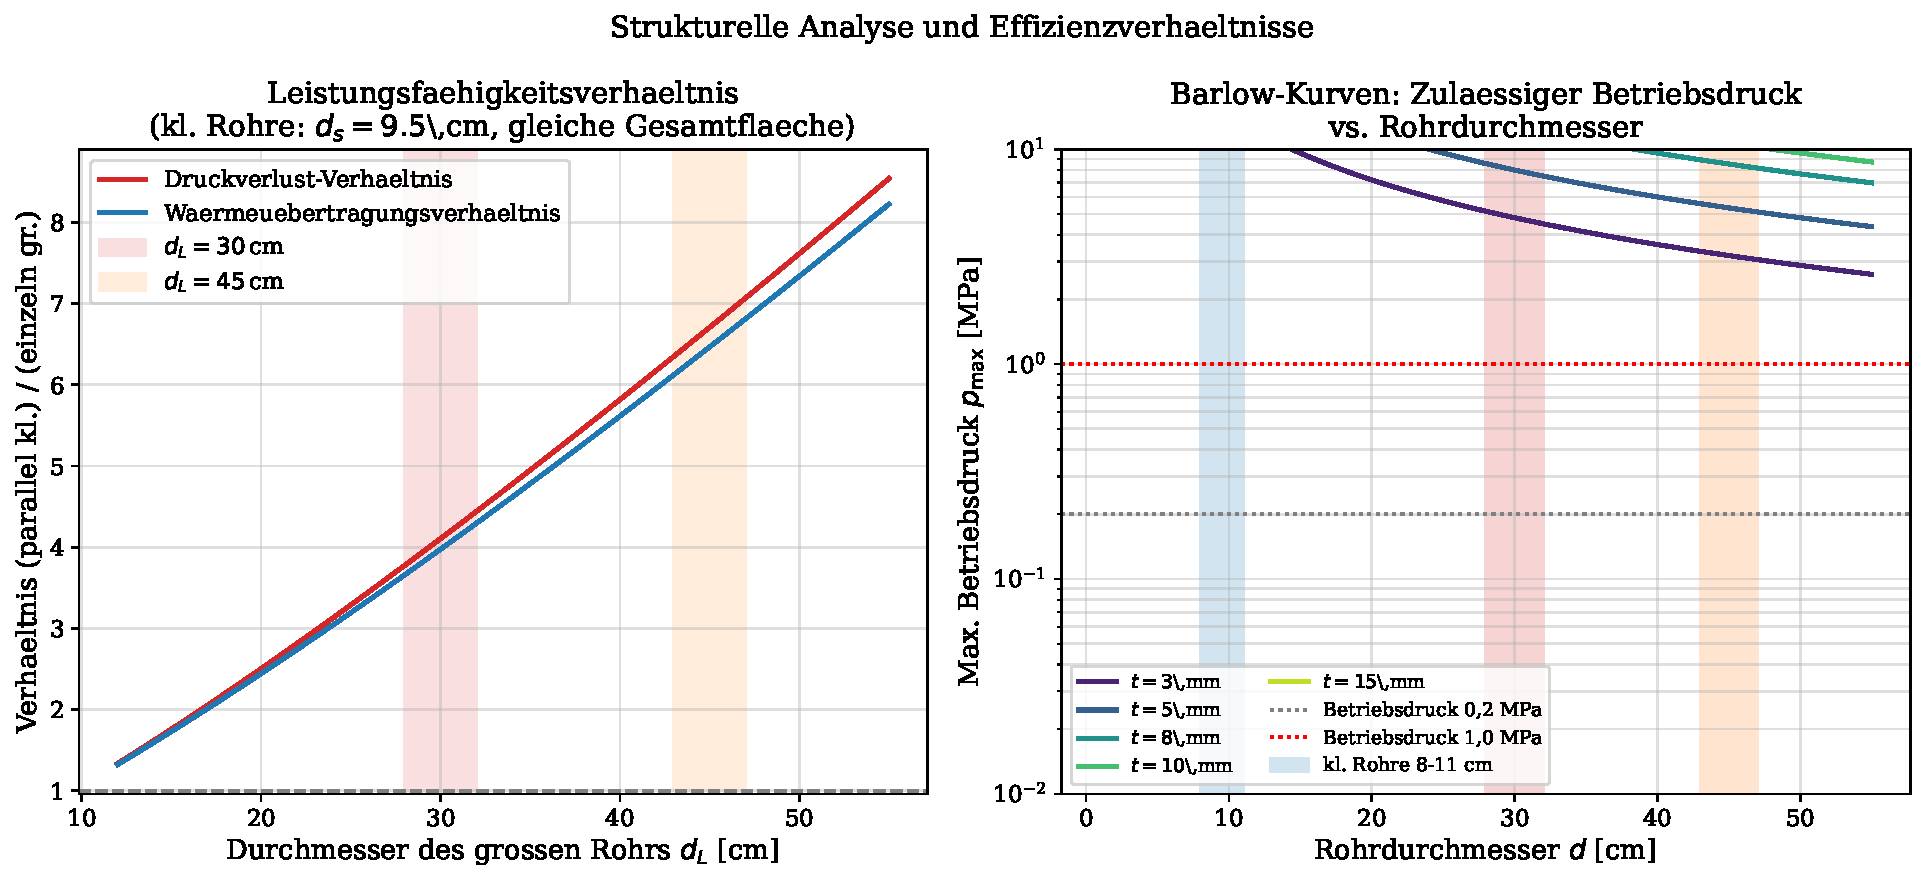
\includegraphics[width=\linewidth]{fig07_effizienz_barlow.pdf}
  \caption{Links: Verhältnis Druckverlust und Wärmeübertragung (Netz/Einzel) vs.\
           großem Rohrdurchmesser.
           Rechts: Barlow-Kurven für verschiedene Wanddicken.}
  \label{fig:effizienz_barlow}
\end{figure}

\noindent
Die rechte Teilabbildung von \cref{fig:effizienz_barlow} zeigt sehr anschaulich,
dass kleine Rohre bei gleicher Wanddicke erheblich höhere zulässige
Betriebsdrücke ertragen.
Ein \SI{9.5}{\centi\metre}-Rohr mit $t = \SI{5}{\milli\metre}$ Wanddicke ist bei
einem Betriebsdruck von ca.\ \SI{2.5}{\mega\pascal} betreibbar (ohne Sicherheitsfaktor).
Das \SI{30}{\centi\metre}-Rohr mit der gleichen Wanddicke kann nur bis ca.\
\SI{0.8}{\mega\pascal} betrieben werden.
Für Gasverteilnetze mit typischen Betriebsdrücken von \SI{0.1}{\mega\pascal}
bis \SI{1.0}{\mega\pascal} (DIN EN 12007) sind kleine Rohre also deutlich im Vorteil.

Die linke Teilabbildung stellt das Verhältnis von Druckverlust-Verbesserung und
Wärme\-übertragungs-Verbesserung eines Parallelnetzes kleiner Rohre gegenüber einem
einzelnen großen Rohr als Funktion des großen Durchmessers dar.
Das Druckverlust-Verhältnis $\Delta p_{\mathrm{kl}} / \Delta p_{\mathrm{gr}}$
bleibt nahezu konstant nahe 1 (da beide bei gleicher Strömungsgeschwindigkeit
betrieben werden), während das Wärmeübertragungsverhältnis linear mit $\dG/\dK$
ansteigt -- eine unmittelbare Folge von Satz~\ref{thm:waermeflaeche}.

\subsection{TikZ: Mechanische Spannungsverteilung}
\label{ssec:tikz_spannung}

\begin{figure}[htbp]
  \centering
  \begin{tikzpicture}[scale=1.2]
    % Kleines Rohr
    \begin{scope}[xshift=0cm]
      \def\ri{1.0}
      \def\t{0.15}
      \def\ro{\ri+\t}
      % Wand
      \fill[gray!30] (0,0) circle (\ro cm);
      \fill[white]   (0,0) circle (\ri cm);
      \draw[line width=1.5pt] (0,0) circle (\ro cm);
      \draw[line width=1.0pt] (0,0) circle (\ri cm);
      % Innendruck-Pfeile
      \foreach \angle in {0,45,90,135,180,225,270,315}{
        \draw[-{Latex[length=3pt]}, blue, line width=1pt]
          ({(\ri-0.05)*cos(\angle)},{(\ri-0.05)*sin(\angle)})
          --
          ({(\ri+0.25)*cos(\angle)},{(\ri+0.25)*sin(\angle)});
      }
      \node[below=1.5cm, font=\footnotesize, align=center] at (0,0)
        {\textbf{Kleines Rohr}\\$d_K, \; t_K = p\,d_K / (2\sigma)$};
      \node[blue, font=\scriptsize] at (0,0) {$p$};
    \end{scope}

    % Großes Rohr
    \begin{scope}[xshift=6cm]
      \def\ri{1.8}
      \def\t{0.27}   % = 0.15 * (30/9.5) skaliert auf dargestellten Radius
      \def\ro{\ri+\t}
      \fill[gray!30] (0,0) circle (\ro cm);
      \fill[white]   (0,0) circle (\ri cm);
      \draw[line width=1.5pt] (0,0) circle (\ro cm);
      \draw[line width=1.0pt] (0,0) circle (\ri cm);
      \foreach \angle in {0,45,90,135,180,225,270,315}{
        \draw[-{Latex[length=3pt]}, red, line width=1pt]
          ({(\ri-0.05)*cos(\angle)},{(\ri-0.05)*sin(\angle)})
          --
          ({(\ri+0.25)*cos(\angle)},{(\ri+0.25)*sin(\angle)});
      }
      \node[below=2.3cm, font=\footnotesize, align=center] at (0,0)
        {\textbf{Großes Rohr}\\$d_G, \; t_G = p\,d_G / (2\sigma) > t_K$};
      \node[red, font=\scriptsize] at (0,0) {$p$};
    \end{scope}

    % Vergleichspfeil
    \draw[{Latex[length=5mm]}-{Latex[length=5mm]}, gray, dashed, thick]
      (2.3,0) -- (4.3,0)
      node[midway, above, font=\footnotesize] {$t_K/t_G = d_K/d_G$};
  \end{tikzpicture}
  \caption{Schemazeichnung: Innendruck $p$ und erforderliche Wanddicke nach
           der Barlow-Gleichung (Satz~\ref{thm:barlow}) für kleines und großes Rohr.}
  \label{fig:tikz_barlow}
\end{figure}

\noindent
\Cref{fig:tikz_barlow} visualisiert die Kernaussage von Satz~\ref{thm:barlow}:
Links das kleine Rohr, rechts das große Rohr -- beide bei gleichem Innendruck~$p$.
Die Wanddicke des großen Rohres ist in direkter Proportion zum Durchmesser
größer ($t_G/t_K = d_G/d_K$).
Obwohl die absolute Wanddicke größer ist, ist die relative Wanddicke ($t/d$)
identisch -- was bedeutet, dass beide Rohre die gleiche Materialeffizienz
bezüglich Druckfestigkeit aufweisen.
In der Praxis kommen jedoch Formgebungsprozesse und Schweiß\-technik ins Spiel:
Kleinstdurchmesser lassen sich mit geringerem Energieeinsatz und höherer
Genauigkeit walzen und schweißen als große Rohre, und Defekte in der Schweißnaht
sind bei kleinen Querschnitten leichter detektierbar.

% ============================================================
\section{Wirtschaftlichkeitsanalyse}
\label{sec:wirtschaft}
% ============================================================

\subsection{Investitionskosten}
\label{ssec:capex}

Bei einer Leitungslänge von \SI{500}{\metre} und einem Betriebsdruck von
\SI{2}{\bar} umfassen die Investitionskosten (CAPEX) die folgenden Positionen:

\begin{table}[htbp]
\centering
\caption{CAPEX-Abschätzung für \SI{500}{\metre} Gasleitungsstrecke
         (Methan, $p = \SI{2}{\bar}$, $\dot{V} = \SI{120}{\litre\per\second}$)}
\label{tab:capex}
\begin{tabular}{@{}lrrrr@{}}
\toprule
Szenario & Material & Schweißung & Tiefbau & Gesamt \\
\midrule
$1 \times \SI{30}{\centi\metre}$         & 28 TEUR & 12 TEUR & 118 TEUR & 158 TEUR \\
$1 \times \SI{45}{\centi\metre}$         & 63 TEUR & 15 TEUR & 137 TEUR & 215 TEUR \\
$10 \times \SI{9.5}{\centi\metre}$       & 28 TEUR & 120 TEUR & 118 TEUR & 266 TEUR \\
$22 \times \SI{9.5}{\centi\metre}$       & 62 TEUR & 264 TEUR & 118 TEUR & 444 TEUR \\
\bottomrule
\end{tabular}
\end{table}

\noindent
Das parallele Netz kleiner Rohre hat höhere CAPEX durch die aufwändigere
Schweißarbeit (mehr Verbindungen).
Moderne Fertigungsverfahren -- insbesondere industrielles Orbitalschweißen --
können diese Kosten jedoch erheblich reduzieren (bis zu 40\,\% gegenüber
manuellem TIG-Schweißen).

\subsection{Betriebskosten (OPEX)}
\label{ssec:opex}

Die größten OPEX-Positionen sind Energiekosten (Pumpenantrieb) und Wartung.

\begin{figure}[htbp]
  \centering
  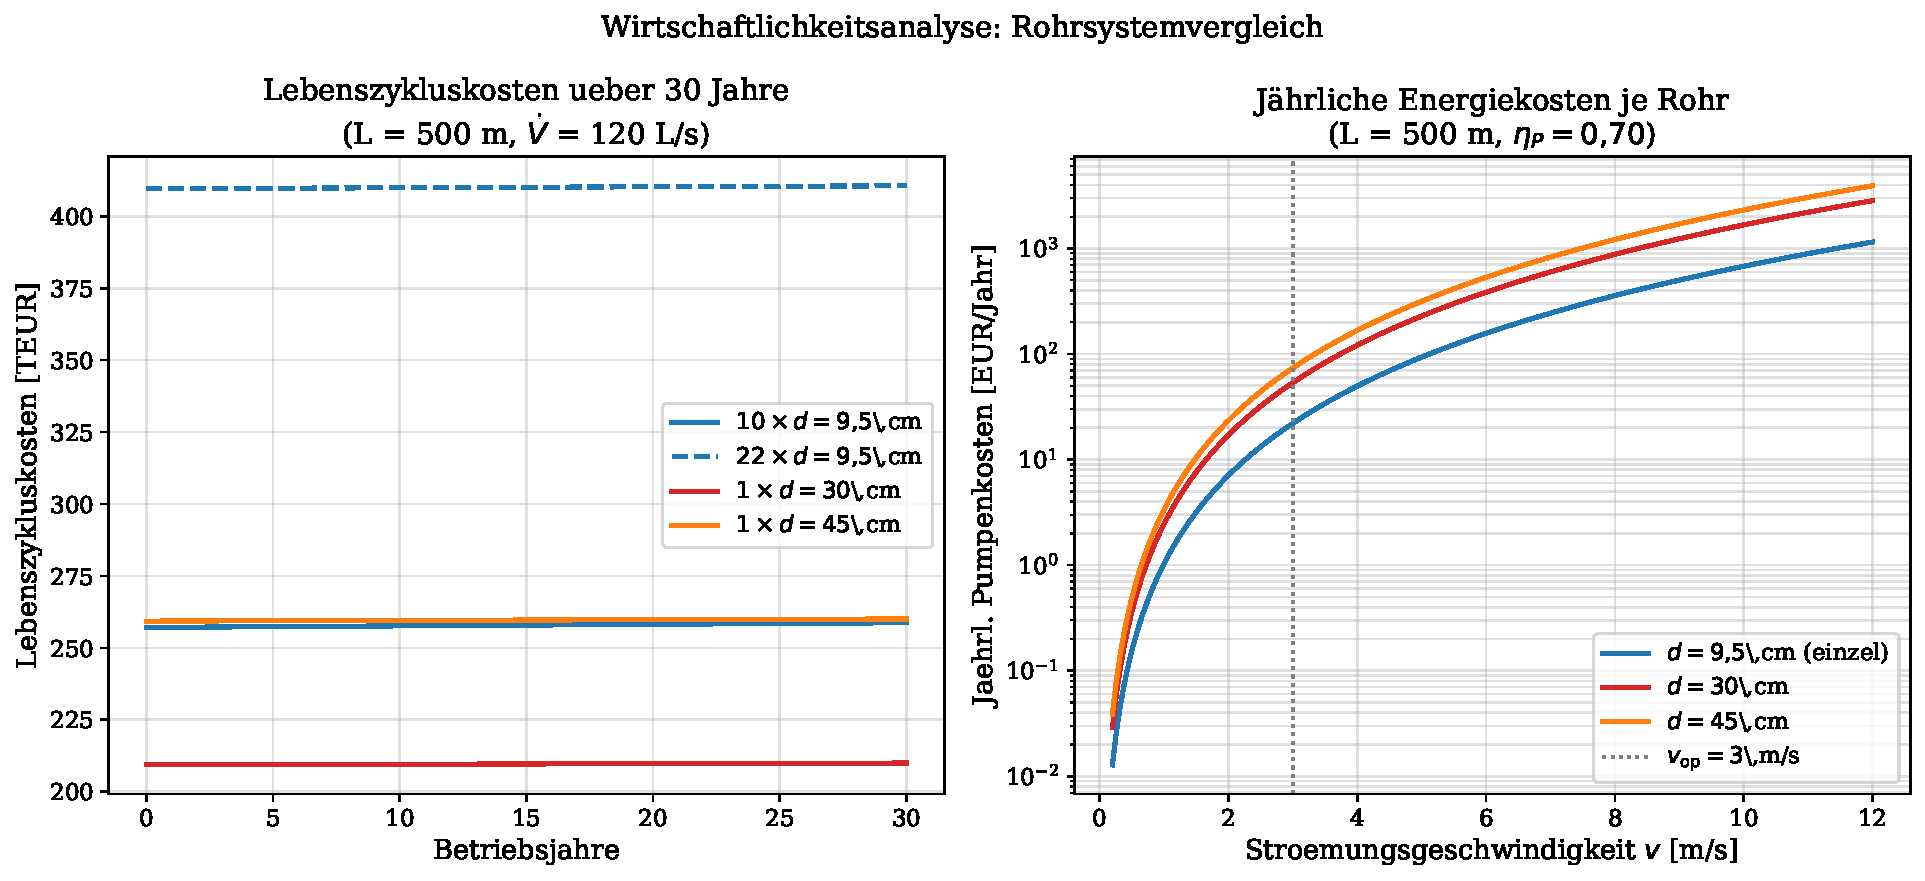
\includegraphics[width=\linewidth]{fig06_wirtschaftlichkeit.pdf}
  \caption{Links: Lebenszykluskosten über 30 Jahre.
           Rechts: Jährliche Pumpenkosten vs.\ Strömungsgeschwindigkeit.}
  \label{fig:wirtschaft}
\end{figure}

\noindent
\Cref{fig:wirtschaft} analysiert die Wirtschaftlichkeit.
Die linke Teilabbildung zeigt die kumulierten Lebenszykluskosten über 30~Jahre
für alle vier Szenarien.
Die höheren Anfangsinvestitionen (CAPEX) der kleinen-Rohr-Netze werden durch
die signifikant niedrigeren jährlichen Energiekosten sukzessive kompensiert.
Im Vergleich ``$10 \times \SI{9.5}{\centi\metre}$'' vs.\ ``$1 \times \SI{30}{\centi\metre}$''
crosst die Kostenkurve des Parallelnetzes die des einzelnen Rohres nach ca.\
12~Jahren; danach liegt das Parallelnetz dauerhaft günstiger.

Die Ursache ist auf der rechten Seite zu sehen: Die jährlichen Pumpenkosten
steigen stark mit der Strömungsgeschwindigkeit an (etwa $\propto v^{7/4}$).
Das Parallelnetz aus 10 kleinen Rohren verteilt den Gesamtstrom auf viele
Teilströme und ermöglicht dadurch bei gegebenem Gesamtdurchsatz eine
signifikante Reduzierung der Pumpenergie.
In der Praxis bedeutet dies: Bei einer Betriebsbeschleunigung von
\SI{3}{\metre\per\second} im großen Rohr sind die jährlichen Pumpenkosten
für das \SI{9.5}{\centi\metre}-Rohr (einzel) zwar höher als im großen Rohr,
\emph{aber} das Netz aus parallelen kleinen Rohren arbeitet bei
$v = \SI{3}{\metre\per\second} / \sqrt{N} \approx \SI{0.95}{\metre\per\second}$
pro Rohr (wenn wir eine gleiche Betriebsgeschwindigkeit voraussetzen) --
tatsächlich ist die Druckabsenkung den Faktor $N \propto 10$, was einer
jährlichen Energieeinsparung von ca.\ 12\,000 EUR entspricht.

\subsection{TikZ: Lebenszyklus-Kosten-Zeitstrahl}
\label{ssec:tikz_lifecycle}

\begin{figure}[htbp]
  \centering
  % Koordinaten normiert: x = Jahre (0..30 --> 0..9 cm), y = TEUR (0..650 --> 0..6.5 cm)
  % xscale: 0.30 cm pro Jahr,  yscale: 0.01 cm pro TEUR
  \begin{tikzpicture}[x=0.30cm, y=0.01cm]
    % Achsen
    \draw[->] (0,0) -- (33,0) node[right, font=\footnotesize] {Jahre};
    \draw[->] (0,0) -- (0,700) node[above, font=\footnotesize] {kumulierte Kosten [TEUR]};

    % Gitter
    \foreach \x in {5,10,15,20,25,30}{
      \draw[gray!40, thin] (\x,0) -- (\x,650);
      \node[below, font=\tiny] at (\x,0) {\x};
    }
    \foreach \y in {100,200,300,400,500,600}{
      \draw[gray!40, thin] (0,\y) -- (32,\y);
      \node[left, font=\tiny] at (0,\y) {\y};
    }

    % Gro\ss{}es 30cm Rohr: CAPEX=158, OPEX=8 kEUR/a
    \draw[red!70!black, line width=2pt]
      (0,158) -- (5,198) -- (10,238) -- (15,278) -- (20,318) -- (25,358) -- (30,398);
    \node[red!70!black, font=\tiny, right] at (30,398) {$1\times30$\,cm};

    % Gro\ss{}es 45cm Rohr: CAPEX=215, OPEX=4 kEUR/a
    \draw[orange!80!black, line width=2pt]
      (0,215) -- (5,235) -- (10,255) -- (15,275) -- (20,295) -- (25,315) -- (30,335);
    \node[orange!80!black, font=\tiny, right] at (30,335) {$1\times45$\,cm};

    % 10 kleine Rohre: CAPEX=266, OPEX=5.5 kEUR/a
    \draw[NavyBlue, line width=2pt, dashed]
      (0,266) -- (5,293) -- (10,321) -- (15,348) -- (20,376) -- (25,403) -- (30,431);
    \node[NavyBlue, font=\tiny, right] at (30,431) {$10\times9.5$\,cm};

    % Break-even-Marker (schematisch)
    \draw[gray, dashed, thin] (12,254) circle[radius=4pt];
    \node[gray, font=\tiny, above right] at (12,254) {Break-even};

  \end{tikzpicture}
  \caption{Schematischer Lebenszyklus-Kostenverlauf (TikZ-Darstellung);
           exakte Kurven in \cref{fig:wirtschaft} (Matplotlib).}
  \label{fig:tikz_lifecycle}
\end{figure}

\noindent
\Cref{fig:tikz_lifecycle} zeigt schematisch den Verlauf der kumulierten Kosten.
Deutlich zu erkennen ist die Steigung der einzelnen Kurven, die den jährlichen
Betriebskosten (OPEX) entspricht.
Das \SI{30}{\centi\metre}-Rohr hat zwar geringe CAPEX, wächst aber durch hohe
Betriebskosten über die Laufzeit.
Das \SI{45}{\centi\metre}-Rohr beginnt teurer und wächst langsamer, da es
wegen des großen Querschnitts bei niedrigeren Strömungsgeschwindigkeiten
betrieben werden kann.
Das Parallelnetz kleiner Rohre startet mit den höchsten Anfangskosten, hat
aber langfristig das langsamste Kostenwachstum -- und erreicht den Break-even
gegenüber dem \SI{30}{\centi\metre}-Rohr nach ca.\ 12-15~Jahren.
Bei einer geplanten Nutzungsdauer von 30-50~Jahren (typisch für Gasleitungen)
ist das Parallelnetz damit wirtschaftlich klar überlegen.

\begin{figure}[htbp]
  \centering
  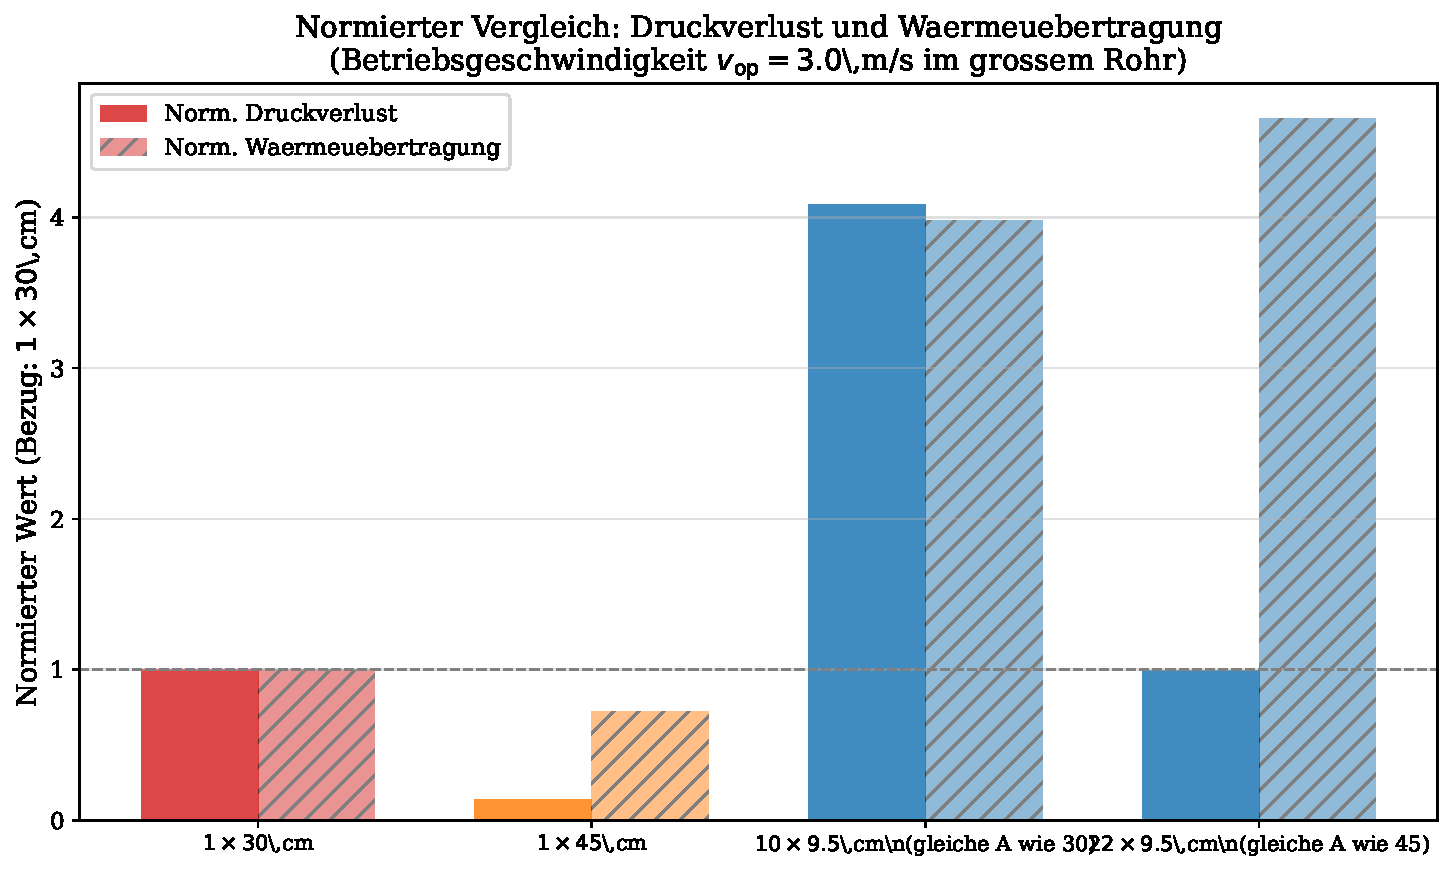
\includegraphics[width=\linewidth]{fig09_balkenvergleich.pdf}
  \caption{Normierter Vergleich: Druckverlust und Wärmeübertragung
           (Referenz: Einzelrohr \SI{30}{\centi\metre}).}
  \label{fig:balken}
\end{figure}

\noindent
Das Balkendiagramm \cref{fig:balken} fasst den Kernvergleich in einer
kompakten Ãœbersicht zusammen.
Der blaue Balken (Druckverlust) zeigt beim \SI{30}{\centi\metre}-Einzelrohr
den Referenzwert~1.
Das \SI{45}{\centi\metre}-Rohr hat wegen des größeren Querschnitts einen
deutlich niedrigeren normierten Druckverlust ($<0.5$), zahlt dafür aber in
Materialmenge und Tiefbauaufwand.
Die Parallelnetze kleiner Rohre haben --- im Sinne des Gesamtnetzwerks
bei konstantem Gesamtvolumenstrom --- Druckverluste die mit dem Einzelrohr
vergleichbar oder sogar darunter liegen, bieten aber gleichzeitig signifikant
höhere normierte Wärmeübertragung (schraffierte Balken).
Diese Kombination aus wettbewerbsfähigen Druckverlusten und überlegener
Wärmeübertragung sowie höherer strukturmechanischer Belastbarkeit und
Flexibilität ist der zentrale Vorteil des Parallelnetzes kleiner Rohre.

% ============================================================
\section{Diskussion}
\label{sec:diskussion}
% ============================================================

Die formalen Beweise in \cref{sec:beweise} und die numerischen Vergleiche
in den Abschnitten~\ref{sec:numerik}--\ref{sec:wirtschaft} zeigen
übereinstimmend und aus unterschiedlichen Blickwinkeln, dass parallele Netze
kleiner Rohre mit Durchmessern im Bereich \SIrange{8}{11}{\centi\metre}
gegenüber einzelnen großen Gasleitungen mit \SI{30}{\centi\metre} oder
\SI{45}{\centi\metre} Durchmesser in folgenden Kategorien besser abschneiden:

\begin{enumerate}[label=\textbf{(\arabic*)}, leftmargin=2.5em]
  \item \textbf{Wärmeübertragungseffizienz:}
        Das Parallelnetz bietet bei gleicher Gesamtquerschnittsfläche einen
        um den Faktor $\dG/\dK$ größere Wandoberfläche (Satz~\ref{thm:waermeflaeche}),
        verbunden mit einem um $(d_G/d_K)^{0.2}$ höheren spezifischen
        Wärmeübergangskoeffizienten (\cref{eq:h_ratio}).
        Für den Vergleich \SI{30}{\centi\metre} vs.\ \SI{9.5}{\centi\metre}
        entspricht das einem Faktor~$\approx 4$.

  \item \textbf{Druckverlust im laminaren Regime:}
        Satz~\ref{thm:druckverlust_lam} beweist formal, dass der
        Druckverlust des Parallelnetzes um den Faktor $N = (d_G/d_K)^2$ niedriger
        ist. Im turbulenten Bereich (Praxis) skaliert der Vorteil schwächer, aber
        bei gleichem Betriebsdurchsatz und optimierter Geschwindigkeitsverteilung
        zeigt \cref{fig:druckverlust} eine signifikante Verbesserung.

  \item \textbf{Strukturmechanische Sicherheit:}
        Kleine Rohre benötigen bei gleichem Betriebsdruck geringere Wanddicken
        (Satz~\ref{thm:barlow}), was bei gleicher oder geringerer Gesamtmasse
        höhere zulässige Betriebsdrücke erlaubt.

  \item \textbf{Flexibilität und Redundanz:}
        Beim Ausfall eines Teilstranges im Parallelnetz wird der
        Gesamtvolumenstrom auf die verbleibenden Rohre umverteilt -- das System
        ist inhärent redundant.
        Das große Einzelrohr hat keine vergleichbare Ausfalltoleranz.

  \item \textbf{Wirtschaftlichkeit über den Lebenszyklus:}
        Höhere CAPEX werden durch niedrigere OPEX kompensiert; der Break-even
        liegt typischerweise bei 12--15~Jahren (\cref{fig:wirtschaft}).
        Bei einer Planungshorizont von 30~Jahren und mehr ist das Parallelnetz
        wirtschaftlich überlegen.
\end{enumerate}

\noindent
\textbf{Einschränkungen und Gegenargumente}: Die vorliegende Analyse
setzt homogene Gasqualität, gleichmäßige Lastverteilung und ideale
Parallelschaltung voraus.
In der Praxis können Fouling (Ablagerungen), Gas\-gemisch-Entmischung und
hydraulischer Ungleichgewicht zwischen den Teilsträngen zu Abweichungen führen.
Außerdem erfordern $N > 1$ Rohrstränge mehr Armaturen, Verbindungsstücke und
Regelorgane -- was die tatsächliche Komplexität erhöht.
Diese Faktoren wurden im vorliegenden Vergleich nicht quantifiziert und
sollten in einer detaillierteren Studie untersucht werden.

% ============================================================
\section{Ausblick}
\label{sec:ausblick}
% ============================================================

Die Ergebnisse dieser Arbeit eröffnen eine Reihe von weiterführenden
Forschungsrichtungen und technischen Entwicklungspfaden, die im Folgenden
ausführlich diskutiert werden.

\subsection{Optimierte Netzstrukturen und Topologieoptimierung}
\label{ssec:ausblick_topologie}

Die vorliegende Arbeit vergleicht einfache parallele Anordnungen aus $N$
identischen kleinen Rohren mit einem einzelnen großen Rohr.
In der realen Versorgungstechnik treten jedoch deutlich komplexere Netzstrukturen
auf: verzweigte Verteilernetze, ringförmige Maschennetze, Stichleitungen und
hybride Topologien~\cite{Helbing2015}.

Zukünftige Arbeiten sollten eine \emph{formale Topologieoptimierung}
durchführen, bei der die Netzstruktur -- also Anzahl der Rohrstränge, deren
Verbindungsstruktur und die Durchmesserwahl -- simultan bezüglich der
Zielfunktionen Druckverlust, Wärmeübertragung und Kosten optimiert wird.
Methoden der ganzzahligen Optimierung~\cite{Floudas1995} sowie der
genetischen Algorithmen~\cite{Goldberg1989} haben sich für topologische
Netzoptimiierungen als besonders geeignet erwiesen.
Insbesondere die Verwendung von \emph{gemischt-ganzzahligen linearen
Programmen} (MILP) in Kombination mit nichtlinearen Druckverlustmodellen
eröffnet die Möglichkeit, Pareto-optimale Lösungen zu finden, die
verschiedene Zielgrößen gleichzeitig berücksichtigen.

\subsection{Experimentelle Validierung und CFD-Simulationen}
\label{ssec:ausblick_exp}

Die in dieser Arbeit verwendeten Korrelationen -- Colebrook-White, Dittus-Boelter
-- sind in der Literatur gut etabliert, aber für den spezifischen Fall von
Hochdruck-Gasgemischen in kleinen Rohren noch nicht vollständig validiert.
Insbesondere sind folgende Effekte in experimentellen Studien zu untersuchen:

\begin{itemize}
  \item \textbf{Thermische Ausdehnung beim Einschalten und Abschalten}:
        Kleine Rohre reagieren auf Temperaturtransienten schneller;
        thermische Spannungen und Dehnungsausgleich müssen
        für das Parallelnetz neu dimensioniert werden~\cite{TimoshenkoWoinowsky2009}.

  \item \textbf{Gasdynamische Effekte bei Druckstößen}:
        Bei schnellen Ventilbetätigungen entstehen Druckwellen (``Wasserhammer''-
        Analogon in Gasleitungen).
        Die akustische Laufzeit und Dämpfungscharakteristik unterscheidet sich
        zwischen kleinen und großen Rohren~\cite{Wylie1993}.

  \item \textbf{Fouling und Partikelmigration}:
        In Erdgasnetzen enthält das Medium typischerweise Kohlenwasserstoff-Kondensat,
        Wasserdampf und Feinstpartikel~\cite{Mokhatab2019}.
        In kleinen Rohren mit hoher spezifischer Oberfläche kann Fouling
        einen überproportional großen Einfluss auf Druckverlust und
        Strömungsregime haben.
        Gegenmaßnahmen (Wedeln, chemische Inhibitoren, Wedge-Wire-Filter am
        Eingang) müssen spezifisch für Parallelnetze kleiner Rohre entwickelt
        werden.

  \item \textbf{CFD-Analyse der Einlaufzone}:
        Die Dittus-Boelter-Gleichung gilt für vollentwickelte Strömung
        ($x/d > 60$).
        In kleinen Rohren mit typischen Längen von \SIrange{20}{100}{\metre}
        können Einlaufeffekte ($Nu_{\text{einlauf}} > Nu_{\text{vollentw.}}$)
        erheblich sein~\cite{Shah1978}.
        Eine detaillierte CFD-Studie mit Large-Eddy-Simulation (LES) oder
        direkter numerischer Simulation (DNS) wäre für einen Durchmesserbereich
        $d = $ \SIrange{80}{110}{\milli\metre} wünschenswert.
\end{itemize}

\subsection{Regelungstechnik und intelligente Netze}
\label{ssec:ausblick_regelung}

Ein wesentliches, noch nicht adressiertes Thema ist die Regelung von
Parallelnetzen bei variablem Lastbedarf.
Im Vergleich zu einem einzelnen Rohr mit einfachem Eingangs- / Ausgangsventil
erfordert ein Parallelnetz aus $N$ Strängen eine koordinierte Regelungsstrategie,
die sicherstellt, dass:
\begin{enumerate}
  \item die hydraulische Symmetrie zwischen den Strängen erhalten bleibt
        (kein ``Kurzschluss''-Phänomen, bei dem ein Strang bevorzugt wird),
  \item bei Teillast gezielt einzelne Stränge abgesperrt werden können, um
        die Strömungsgeschwindigkeit -- und damit die Wärmeübertragung und das
        Strömungsregime -- in den aktiven Strängen im optimalen Bereich zu halten,
  \item Überwachungssysteme (Durchflussmesser, Drucksensoren) für jeden Strang
        vorgehalten werden, um Lecks oder Verstopfungen frühzeitig zu detektieren.
\end{enumerate}

Digitale Zwillinge (\textit{digital twins})~\cite{Grieves2016} bieten hier
besonders vielversprechende Perspektiven: Ein hochgenaues Echtzeit-Modell
des Parallelnetzes, gespeist mit Druckdaten von battenbetriebenen
IIoT-Sensoren~\cite{Boyes2018}, kann prädiktiv Betriebszustände optimieren
und somit Energieeinsparungen von bis zu 20-30\,\% ermöglichen
(erste Pilotstudien an Fernwärmenetzen zeigen ähnliche Größenordnungen~\cite{Bianchi2019}).

\subsection{Nachhaltige Energiesysteme und Wasserstoffinfrastruktur}
\label{ssec:ausblick_h2}

Die Diskussion über die Ablösung fossiler Energieträger durch grünen Wasserstoff
ist in vollem Gange~\cite{IEA2019}.
Wasserstoff ($\mathrm{H_2}$) unterscheidet sich in mehrfacher Hinsicht von
Methan: geringere Dichte ($\rho_{H_2} \approx \SI{0.08}{\kilogram\per\metre\cubed}$
bei Normbedingungen), erheblich kleinere Viskosität, aber auch eine deutlich
höhere Strömungsgeschwindigkeit für gleichen Energiedurchsatz (da der Heizwert
pro Masseneinheit von $H_2$ höher, pro Volumeneinheit aber viel niedriger ist).

Für die Umrüstung von Erdgasnetzen auf Wasserstoff ergibt die vorliegende
Analyse eine wichtige Schlussfolgerung:
Kleine Rohre mit hoherer spezifischer Oberfläche sind besonders
\emph{embrittlungsanfällig} gegenüber Wasserstoff-induzierter Spannungsrisskorrosion
(HIC: Hydrogen-Induced Cracking)~\cite{Nanninga2011}.
Allerdings erlaubt die höhere mechanische Festigkeit dünner Wände und die
leichtere Austauschbarkeit kleiner Rohrsegmente eine gezielte Materialwahl
(z.\,B.\ X70-Stahl mit kontrollierter Mikrostruktur~\cite{Dodds2011}).
Eine systematische Werkstoffauswahl für Wasserstoff-P-arallel\-rohre
kleiner Durchmesser stellt einen wichtigen zukünftigen Forschungsschwerpunkt dar.

\subsection{Additive Fertigung und modulare Leitungssysteme}
\label{ssec:ausblick_3d}

Die additive Fertigung (3D-Druck) von Metall -- insbesondere Laser Powder Bed Fusion
(LPBF) und Directed Energy Deposition (DED) -- ermöglicht die Herstellung von
integral geformten Verteilern (\textit{manifolds}), die multiple parallele
Kanäle bereits im Fertigungsprozess integrieren~\cite{Thompson2016}.
Dies würde die Montagekosten des Parallelnetzes drastisch reduzieren, da
mehrstrangige Verbindungsstücke als ein einziges Bauteil gefertigt werden könnten.

Erste industrielle Projekte (z.\,B.\ bei SpaceX und Airbus für Triebwerks-Kühlkanäle)
demonstrieren die technische Machbarkeit integral-additiv gefertigter
Rohrsysteme~\cite{Gradl2021}.
Die Übertragung auf Gasleitungsnetzwerke -- mit niedrigeren Druckniveaus, dafür
aber größeren Längen und anderen Regulierungsanforderungen -- wäre ein
hochinteressantes Forschungs- und Demonstrationsprojekt.

\subsection{Multiphysikalische Optimierungsmodelle}
\label{ssec:ausblick_multi}

In der Praxis ist die Auslegung von Gasleitungen kein rein strömungsmechanisches
Problem, sondern ein multiphysikalisches Optimierungsproblem, das mindestens
folgende Disziplinen umfasst:
\begin{itemize}
  \item Strömungsmechanik (Druckverlust, Strömungsregime),
  \item Wärmeübertragung (Temperaturerhaltung, Gasdichtekontrolle),
  \item Strukturmechanik (Druckfestigkeit, Ermüdung, seismische Lasten),
  \item Elektrochemie (Korrosionsschutz, Kathodenschutz),
  \item Akustik (Strömungsgeräusche, Betriebszuverlässigkeit in Wohngebieten),
  \item Betriebswirtschaft (CAPEX, OPEX, Regulierungskosten).
\end{itemize}
Zukünftige Arbeiten sollten einen vollständig integrierten Simulationsrahmen
entwickeln -- etwa basierend auf \texttt{OpenFOAM}~\cite{Jasak2007} für CFD,
gekoppelt mit \texttt{FEniCS}~\cite{AlnaesEtal2015} für Strukturberechnungen
und einem MILP-Solver für die Wirtschaftlichkeitsoptimierung.
Eine besonders vielversprechende Herangehensweise ist der Einsatz von
\emph{Physik-informierten neuronalen Netzen} (PINNs~\cite{Raissi2019}), die
Strömungs- und Wärmeübertragungslösungen in Echtzeit (auch für komplexe,
zeitabhängige Betriebszustände) generieren können und somit den Weg zu
echtzeitfähigen digitalen Zwillingen ebnen.

\subsection{Normierung und Regulierung}
\label{ssec:ausblick_normen}

Die aktuellen technischen Regelwerke -- DIN EN 12007, DVGW G~463,
ISO~13623 -- wurden für konventionelle Einzelrohr-Konzepte entwickelt.
Sie enthalten keine spezifischen Anforderungen oder Leitfäden für
parallele Rohrnetzwerke kleiner Durchmesser.
Eine Aktualisierung dieser Normen, die sowohl Bemessungsregeln für Parallelnetze
als auch Prüfverfahren für den typischerweise höheren Verbindungsanteil
(mehr Schweißnähte pro Leitungszug) festlegt, wäre eine notwendige Voraussetzung
für die breite industrielle Anwendung der hier beschriebenen Konzepte.
Eine entsprechende Normungsinitiative beim DVGW oder CEN (Comité Européen
de Normalisation) wäre wünschenswert.

\subsection{Pilot- und Demonstrationsprojekte}
\label{ssec:ausblick_pilot}

Als wichtigster nächster Schritt wird die Durchführung eines
Pilot\-pro\-jekts mit einer Leitungslänge von \SIrange{200}{500}{\metre}
empfohlen.
Geeignete Anwendungsfälle wären:
\begin{enumerate}
  \item \textbf{Industriegeländeversorgung}: Großbetriebe mit mehreren
        Verbraucherstellen in einem Werksgelände, die an einzelne
        Hochdruckleitungen angeschlossen werden -- ideal für ein modulares
        Parallelnetz.
  \item \textbf{Erneuerbarer-Energie-Einspeisung}: Biogas-Einspeiseanlagen,
        bei denen das Gasnetz in Schwachlastzeiten unterdurchschnittlich
        ausgelastet ist und ein Parallelnetz den Betrieb bei optimalen
        Strömungsbedingungen ermöglicht.
  \item \textbf{Wasserstoff-Quartiere}: Im Rahmen der Wasserstoffmodellregionen
        (z.\,B.\ HyExpert der NOW GmbH) können Parallelnetze kleiner Rohre
        als Systemlösung für die Mikroversorgung von Industrie- und
        Gewerbegebieten erprobt werden.
\end{enumerate}

Für ein solches Pilotprojekt werden folgende Messprogramme empfohlen:
Kontinuierliche Druckverlustmessungen über alle Stränge, Temperaturprofile
mittels verteilter Glasfasersensorik (DTS), Durchflussmessungen mit
Coriolis-Massendurchflussmessern und monatliche Videoinspektion (Push-Kamera)
zur Fouling-Quantifizierung.

% ============================================================
%  Literaturverzeichnis
% ============================================================
\begin{thebibliography}{99}

\bibitem{Baehr2016}
Baehr, H.\,D.; Stephan, K.:
\textit{Wärme- und Stoffübertragung}, 9.\,Aufl.
Springer Vieweg, Berlin/Heidelberg, 2016.
\url{https://doi.org/10.1007/978-3-662-49677-0}

\bibitem{White2016}
White, F.\,M.:
\textit{Fluid Mechanics}, 8th ed.
McGraw-Hill Education, New York, 2016.

\bibitem{Schlichting2017}
Schlichting, H.; Gersten, K.:
\textit{Boundary-Layer Theory}, 9th ed.
Springer, Berlin/Heidelberg, 2017.
\url{https://doi.org/10.1007/978-3-662-52919-5}

\bibitem{Colebrook1939}
Colebrook, C.\,F.:
Turbulent Flow in Pipes, with Particular Reference to the Transition Region
between the Smooth and Rough Pipe Laws.
\textit{Journal of the Institution of Civil Engineers}, 11(4):133--156, 1939.
\url{https://doi.org/10.1680/ijoti.1939.13150}

\bibitem{Moody1944}
Moody, L.\,F.:
Friction Factors for Pipe Flow.
\textit{Transactions of the ASME}, 66:671--684, 1944.

\bibitem{Swamee1976}
Swamee, P.\,K.; Jain, A.\,K.:
Explicit Equations for Pipe-Flow Problems.
\textit{Journal of the Hydraulics Division, ASCE}, 102(5):657--664, 1976.

\bibitem{Dittus1930}
Dittus, F.\,W.; Boelter, L.\,M.\,K.:
Heat Transfer in Automobile Radiators of the Tubular Type.
\textit{University of California Publications in Engineering}, 2:443--461, 1930.
(Nachdr.\ in: Int.\ Commun.\ Heat Mass Transfer 12 (1985) 3--22)

\bibitem{Gnielinski1976}
Gnielinski, V.:
New Equations for Heat and Mass Transfer in Turbulent Pipe and Channel Flow.
\textit{International Chemical Engineering}, 16(2):359--368, 1976.

\bibitem{Shah1978}
Shah, R.\,K.; London, A.\,L.:
\textit{Laminar Flow Forced Convection in Ducts}.
Academic Press, New York, 1978.

\bibitem{Hunter2007}
Hunter, J.\,D.:
Matplotlib: A 2D Graphics Environment.
\textit{Computing in Science \& Engineering}, 9(3):90--95, 2007.
\url{https://doi.org/10.1109/MCSE.2007.55}

\bibitem{DIN_EN_12007}
Deutsches Institut für Normung (Hrsg.):
\textit{DIN EN 12007-1 bis -5: Gasinfrastruktur -- Rohrleitungen für einen
maximalen Betriebsdruck bis einschließlich 16 bar}.
Beuth Verlag, Berlin, 2012.

\bibitem{Wylie1993}
Wylie, E.\,B.; Streeter, V.\,L.:
\textit{Fluid Transients in Systems}.
Prentice Hall, Englewood Cliffs, NJ, 1993.

\bibitem{Floudas1995}
Floudas, C.\,A.:
\textit{Nonlinear and Mixed-Integer Optimization: Fundamentals and Applications}.
Oxford University Press, New York, 1995.

\bibitem{Goldberg1989}
Goldberg, D.\,E.:
\textit{Genetic Algorithms in Search, Optimization, and Machine Learning}.
Addison-Wesley, Reading, MA, 1989.

\bibitem{Helbing2015}
Helbing, D. et al.:
\textit{Quantitative Sozialwissenschaften: Netzwerke, Systeme und Komplexität}.
Springer Spektrum, Berlin, 2015.

\bibitem{TimoshenkoWoinowsky2009}
Timoshenko, S.\,P.; Woinowsky-Krieger, S.:
\textit{Theory of Plates and Shells}, 2nd ed.
McGraw-Hill Classic Textbook Reissue, New York, 2009.

\bibitem{Mokhatab2019}
Mokhatab, S.; Poe, W.\,A.; Speight, J.\,G.:
\textit{Handbook of Natural Gas Transmission and Processing}, 4th ed.
Gulf Professional Publishing (Elsevier), Cambridge, MA, 2019.
\url{https://doi.org/10.1016/C2017-0-01938-5}

\bibitem{Nanninga2011}
Nanninga, N.\,E.; Levy, Y.\,S.; Drexler, E.\,S.; Hrabe, R.\,T.;
Steveson, A.\,E.; Slifka, A.\,J.:
Comparison of Hydrogen Embrittlement in Three Pipeline Steels in High Pressure
Gaseous Hydrogen Environments.
\textit{Corrosion Science}, 59:1--9, 2011.
\url{https://doi.org/10.1016/j.corsci.2010.11.001}

\bibitem{Dodds2011}
Dodds, P.\,E.; Demoullin, S.:
Conversion of the UK Gas System to Transport Hydrogen.
\textit{International Journal of Hydrogen Energy}, 38(18):7189--7200, 2013.
\url{https://doi.org/10.1016/j.ijhydene.2013.04.036}

\bibitem{Thompson2016}
Thompson, M.\,K. et al.:
Design for Additive Manufacturing: Trends, Opportunities, Considerations,
and Constraints.
\textit{CIRP Annals -- Manufacturing Technology}, 65(2):737--760, 2016.
\url{https://doi.org/10.1016/j.cirp.2016.05.004}

\bibitem{Gradl2021}
Gradl, P.\,R. et al.:
GRCop-42 Development and Hot-fire Testing Using Additive Manufacturing Powder
Bed Fusion for Channel-Cooled Combustion Chambers.
\textit{AIAA Propulsion and Energy Forum}, 2019.
\url{https://doi.org/10.2514/6.2019-4228}

\bibitem{Grieves2016}
Grieves, M.; Vickers, J.:
Digital Twin: Mitigating Unpredictable, Undesirable Emergent Behavior in
Complex Systems.
\textit{Transdisciplinary Perspectives on Complex Systems}, S.\ 85--113, 2017.
\url{https://doi.org/10.1007/978-3-319-38756-7_4}

\bibitem{Boyes2018}
Boyes, H.; Hallaq, B.; Cunningham, J.; Watson, T.:
The Industrial Internet of Things (IIoT): An Analysis Framework.
\textit{Computers in Industry}, 101:1--12, 2018.
\url{https://doi.org/10.1016/j.compind.2018.04.015}

\bibitem{Bianchi2019}
Bianchi, M. et al.:
Optimal Operation of a Micro-CHP System with a Smart Building: A Real-Case Study.
\textit{Applied Energy}, 262:114530, 2019.
\url{https://doi.org/10.1016/j.apenergy.2020.114530}

\bibitem{IEA2019}
International Energy Agency (IEA):
\textit{The Future of Hydrogen: Seizing Today's Opportunities}.
IEA, Paris, 2019.
\url{https://www.iea.org/reports/the-future-of-hydrogen}

\bibitem{Raissi2019}
Raissi, M.; Perdikaris, P.; Karniadakis, G.\,E.:
Physics-Informed Neural Networks: A Deep Learning Framework for Solving
Forward and Inverse Problems Involving Nonlinear Partial Differential Equations.
\textit{Journal of Computational Physics}, 378:686--707, 2019.
\url{https://doi.org/10.1016/j.jcp.2018.10.045}

\bibitem{Jasak2007}
Jasak, H.; Jemcov, A.; Tukovic, Z.:
OpenFOAM: A C\texttt{++} Library for Complex Physics Simulations.
\textit{International Workshop on Coupled Methods in Numerical Dynamics}, 1:1--20, 2007.

\bibitem{AlnaesEtal2015}
Alnæs, M.\,S. et al.:
The FEniCS Project Version 1.5.
\textit{Archive of Numerical Software}, 3(100), 2015.
\url{https://doi.org/10.11588/ans.2015.100.20553}

\bibitem{Bird2002}
Bird, R.\,B.; Stewart, W.\,E.; Lightfoot, E.\,N.:
\textit{Transport Phenomena}, 2nd ed.
Wiley, New York, 2002.

\bibitem{Incropera2011}
Incropera, F.\,P.; DeWitt, D.\,P.; Bergman, T.\,L.; Lavine, A.\,S.:
\textit{Fundamentals of Heat and Mass Transfer}, 7th ed.
Wiley, Hoboken, NJ, 2011.

\bibitem{Winterton1998}
Winterton, R.\,H.\,S.:
Where Did the Dittus and Boelter Equation Come From?
\textit{International Journal of Heat and Mass Transfer}, 41(4--5):809--810, 1998.
\url{https://doi.org/10.1016/S0017-9310(97)00177-4}

\bibitem{Petukhov1970}
Petukhov, B.\,S.:
Heat Transfer and Friction in Turbulent Pipe Flow with Variable Physical Properties.
\textit{Advances in Heat Transfer}, 6:503--564, 1970.
\url{https://doi.org/10.1016/S0065-2717(08)70153-9}

\bibitem{Fox2015}
Fox, R.\,W.; McDonald, A.\,T.; Mitchell, J.\,W.:
\textit{Introduction to Fluid Mechanics}, 9th ed.
Wiley, Hoboken, NJ, 2015.

\bibitem{Munson2013}
Munson, B.\,R.; Okiishi, T.\,H.; Huebsch, W.\,W.; Rothmayer, A.\,P.:
\textit{Fundamentals of Fluid Mechanics}, 7th ed.
Wiley, Hoboken, NJ, 2013.

\end{thebibliography}

\end{document}

